\chapter{螺管范例,HTS磁体和结论}
\section{引言}
本章包括三个部分。第一部分给出多个螺管磁体范例,各范例均有问题与解答(Q/A)。
第二部分讨论HTS磁体应用及其前景。
最后有一个简明的结论性评论。

这里描述和研究的四个螺管磁体范例的选取,不是因为他们特别重要或唯一---
没有哪个磁体系统是唯一的,不过对某些人而言,每一个磁体都是唯一的。
选取这几个例子,主要还是因为作者对这些磁体的熟悉。
在描述部分之后的Q/A部分,前面七章涉及的设计和运行的若干要点,再次提出。

这里,我们再次强调一下第一章中已经阐述过的我们的基本哲学:
任何问题,需要数值解的,首先应该使用经得起数值解检验的简化模型得到近似估计。
近似估计快速告诉磁体设计者磁体是否在正确的轨道上。
对于任何简单或复杂的磁体,该工作都很重要。
 “创新”磁体的想法通常始于个人。
 为了评估这个想法是否切合实际并且值得与同事进一步深入研究甚至组建设计团队,
 发起人必须首先计算设计和运行关键参数的大概值(第2-8章所述),从简单参数如总安匝数、整体运行电流密度、磁体尺寸和重量、导体总长度,到更复杂的如稳定性和保护、力和低温要求。
 这里的关键词是近似:在磁体项目的后期阶段,设计团队的专家将使用复杂的程序来计算准确的参数值。
 将确切的值留给专家,但要准备好确认他们确实属于独立计算的近似数字范围。
 作者希望在研究了第2-8章后,读者---电磁场、应力、低温、甚至材料领域的专家---
 将能够处理下面提出的四个磁体示例中包含的大多数问题。


\section{螺管磁体示例}
实例中描述和研究的四个螺管磁体是:
1)  由一个大型超导磁体和一个电阻性内插磁体组成的混合磁体;
2) 钢板上的磁体;
3) 一个由螺管磁体产生的磁场悬浮起来的HTS板(盘片);
4) 层叠HTS环组成的“螺管”磁体,HTS环由块材加工或图层导体板构成。 


\subsection{例A:串联混合磁体}
NHMFL建造的中心轴向场35-40 T(取决于室温孔大小,32-50 mm)的高场磁体,由
一个超导磁体和一个5线圈高均匀电阻性(水冷)内插磁体组成。
因为超导磁体和5线圈电阻性内插磁体电气上串联且由同一个DC电源供电,
磁体被称为“串联混合磁体”(series-connected-hybrid, SCH)。
SCH产生的中心场大于NHMFL所有的电阻性磁体的磁场(35 T)或全超导磁体的磁场(21 T)。
图9.1给出了SCH磁体的剖面示意图---
参数值与SCH磁体的最终采纳值略有不同。

SCH还包括一个薄($\alpha\simeq 1$)的超导屏蔽线圈,绕组半径约1 m,图中未画出。
屏蔽线圈的反极性的,用以减小SCH磁体的边缘场。
在Q/A部分,我们将计算超导屏蔽线圈要求的安匝数近似值。
同时,我们还将设计可作为技术备选的钢圆柱壳屏蔽系统。
\begin{figure}[htbp]
	\centering
	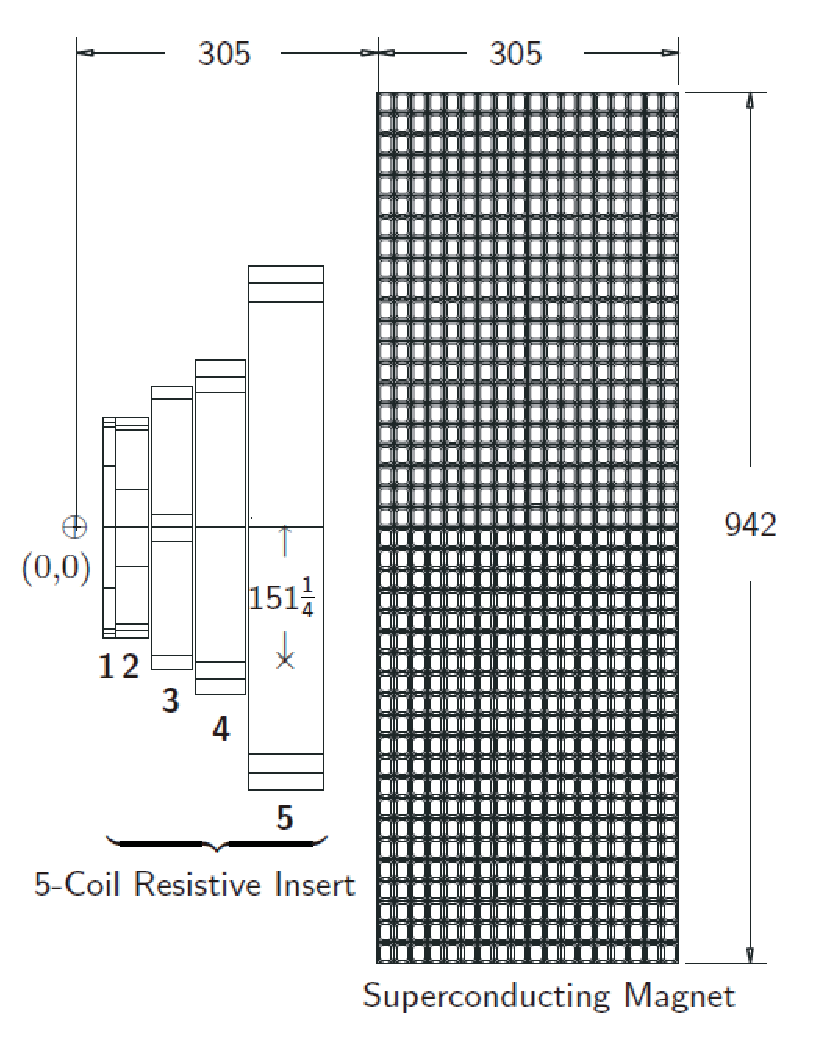
\includegraphics[scale=0.6]{chpt9/figs/fig9.1.eps}
	\caption{NHMFL的SCH磁体的一半结构的剖视图---
		半径约1 m的超导屏蔽线圈未画出。绕组的尺度为近似值,以mm为单位;
	线圈5的$\times$号表示它在故障模式后的磁场中心---将在Q/A部分讨论。}
\end{figure}

\begin{figure}[htbp]
	\centering
	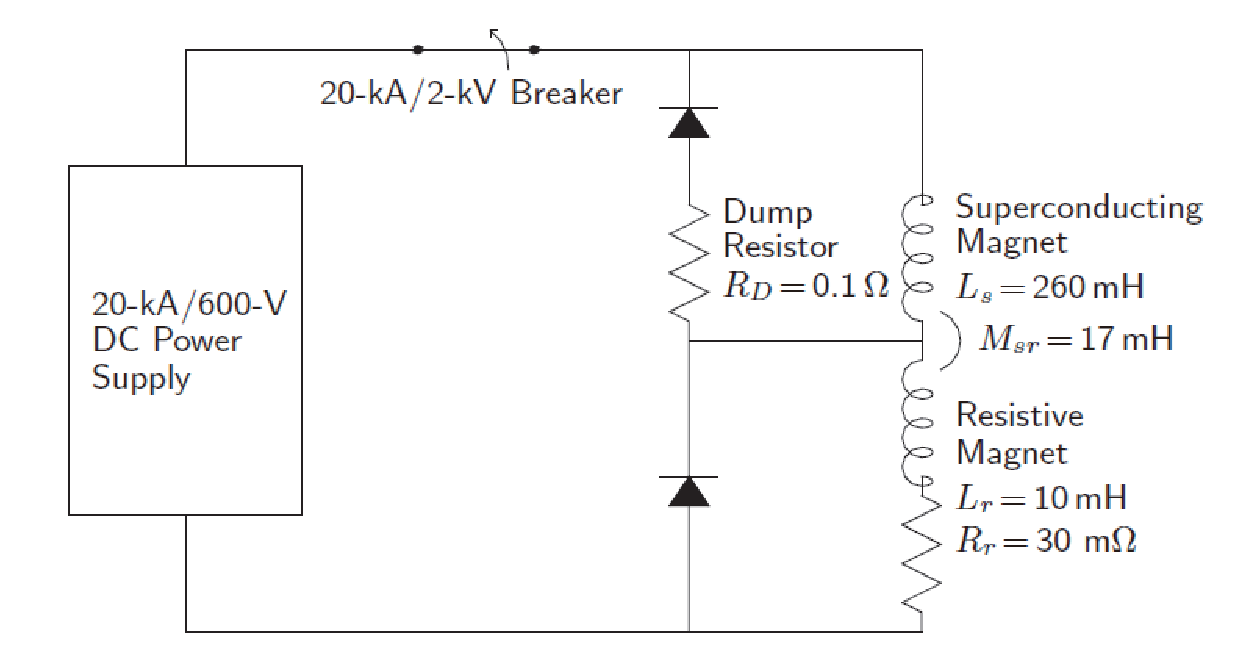
\includegraphics[scale=0.6]{chpt9/figs/fig9.2.eps}
	\caption{SCH磁体的等效电路图。[NHMFL授权使用,2005]}
\end{figure}

图9.2给出了SCH的等效电路图。其中,超导磁体(自感$L_s$=260 mH)与电阻性磁体(自感$L_r$=10 mH,电阻$R_r$=30 m$\Omega$)串联。
磁体由一个20 kA/600 V电源供电。
保护方面,超导磁体用$R_D$=0.1 $\Omega$泄放电阻和二极管串联组作为旁路;
电阻性磁体使用二极管旁路。
(假设两个二极管都是理想的,即正向电阻为零,反向电阻无穷大。)
如图9.2所示,两个磁体间互感$M_{sr}$为17 mH。
在任一磁体异常时,打开20 kA/2 kV断路器。

表9.1列出了超导磁体和该磁体最内层使用的CIC导体的关键参数值。
其中的$A_{sc},A_{\bar{m}},A_{m},A_{cl}$分别是$\mathrm{Nb_3 Sn}$ CIC导体的截面、非基底金属截面、基底金属(铜)截面、4.5 K超临界氦截面。

表9.1.。。。。。。。。。。。。。。

\subsubsection{Q/A A:SCH超导磁体}
\textbf{a) 总体电流密度}\qquad 超导磁体在其运行电流$I_{op}$=20 kA时的总体临界电流密度$\lambda J_{op}$是多少?

\textbf{解:}应用方程3.108a,代入$N$=756和$I=I_{op}$=20 kA,我们得到:
\begin{align*}% page548 第1个
\lambda J_{op}&=\frac{NI}{2b(a_2-a_1)}\\ \tag{3.108a}
&=\frac{756(20\times10^3\ \mathrm{A})}{(942.0\ \mathrm{mm})(610.1\ \mathrm{mm}-305.0\ \mathrm{mm})}=52.6\ \mathrm{A/mm^2}
\end{align*}

\textbf{b) 中心场}\qquad 超导磁体在$I_{op}$=20 kA时,在中心位置产生的磁场(磁感应强度)$B_z(0,0)$是多少?

\textbf{解:}类似的,由表9.1,我们有$\alpha=$1220.2/610.0=2.00;$\beta$=942.0/610.0=1.544。
使用方程3.110,有:
\begin{align*}% page548 第3个
B_{z}(0,0)=\frac{\mu_oNI}{2a_1(\alpha-1)}\ln(\frac{\alpha+\sqrt{\alpha^2+\beta^2}}{1+\sqrt{1+\beta^2}}) \tag{3.110}
\end{align*}

于是,
\begin{align*}% page548 第4个
B_z(0,0)&=\frac{(4\pi\times10^{-7}\ \mathrm{H/m})(756)(20\times10^3\ \mathrm{A})}{(0.610\ \mathrm{m})(2.00-1)}\ln(\frac{2.00+\sqrt{(2.00)^2+(1.544)^2}}{1+\sqrt{1+(1.544)^2}})\\
&=14.52\ \mathrm{T}
\end{align*}

\textbf{c) 中平面径向场}\qquad 超导磁体在中平面($z=0$)的$R=a_2$处产生的磁场的径向分量$B_r(z=0,r=2a_2)$是多少?

\textbf{解:}理想螺管磁体或嵌套线圈磁体产生的磁场的径向分量关于中平面对称,所以总是零:$B_r(0,a_2)=0$

\textbf{d) 电感}\qquad 使用方程3.81和3.14计算磁体自感$L_s$的近似值。如前所述,准确值是260 mH。

\textbf{解:}使用方程3.81和3.14,$\mathcal{L}(\alpha=2.00,\beta=1.544)\simeq 1.2$,我们有:
\begin{align*}% page548 第5个
L&=\mu_oa_1N^2\ \mathcal{L}(\alpha,\beta) \\\tag{3.81}
L_s&=(4\pi\times10^{-7}\ \mathrm{H/m})(0.305\ \mathrm{m})(756)^2(1.2)=263\ \mathrm{mH}
\end{align*}

\textbf{e) 储存的磁能}\qquad 超导磁体在运行电流$I_{op}$=20 kA时储存的总磁能$E_{ms}$是多少?

\textbf{解:}此处我们必须考虑互感的影响。所以:
\begin{align*}% page548 第7个
E_{ms}=&\frac{1}{2}(L_s+M_{sr})I_{op}^2\\
=&\frac{1}{2}(260\ \mathrm{mH}+17\ \mathrm{mH})(20\ \mathrm{kA})^2=55.4\ \mathrm{MJ}
\end{align*}

\textbf{f) 二极管}\qquad 解释与电阻$R_D$串联的二极管的两个功能。

\textbf{解:}反向串联的二极管有两个作用:1) 当磁体励磁时,防止电流通过$R_D$,即令100\%的电源电流都进入磁体;
2) 当开关打开时,允许电流通过$R_D$放电。

\textbf{g) 充电电压}\qquad 恒充电速率400 A/s,$dI_s/dt=dI_r/dt=dI_S/dt$=400 A/s,其中,$I_s$是通过超导
磁体的电流,$I_r$是通过电阻性磁体的电流,$I_S$是电源电流。那么,$I_s=I_r=I_S$=10 kA时,要求的电源电压$V_S$是多少?

\textbf{解:}电源电压为:
\begin{align*}% page549 第1个
V_S&=L_s\frac{dI_s}{dt}+M_{sr}\frac{dI_r}{dt}+M_{sr}\frac{dI_s}{dt}+L_r\frac{dI_r}{dt}+R_rL_r\\
&=(L_s+2M_{sr}+L_r)\frac{dI_s}{dt}+R_rI_S \tag{g.1}
\end{align*}

代入合适的值,有:
\begin{align*}% page549 第3个
V_S=(260\ \mathrm{mH}+2\times17\ \mathrm{mH}+10\ \mathrm{mH})(400\ \mathrm{A/s})+(30\ \mathrm{m\Omega})(10\ \mathrm{kA})=421.6\ \mathrm{kA}
\end{align*}

\textbf{h) 功率}\qquad 当充电速率为$dI_S/dt$=400 A/s,$I_S$=10 kA时,电源供给磁体(含超导和电阻部分)的总的瞬时功率$P_S$为多少?

\textbf{解:}如\textbf{g)},我们有:
\begin{align*}% page549 第4个
V_S&=(L_s+2M_{sr}+L_r)\frac{dI_S}{dt}+R_rI_S\\ \tag{g.1}
&=421.6\ \mathrm{V}
\end{align*}

$P_S=V_S I_S$;于是,$P_S$=4.216 MW。
我们注意到,4.216 MW中的1.216 MW[=4.216 MW-(30 m$\Omega$)$\times(10\ \mathrm{kA})^2$]
是无功功率,即存储于两个磁体中的磁能。
随着电源的电流减为零,磁能会“返回”到电源中。

\textbf{i) 600 V电源电压}\qquad 证明在这个电流增长率(400 A/s)下,电源
最大电压600 V在$I_S\simeq$16 kA时达到。

\textbf{解:}要求的总感性电压$V_{ind}$为:
\begin{align*}% page550 第1个
V_{ind}=(L_s+2M_{sr}+L_r)\frac{dI_S}{dt}
\end{align*}
其中,在$dI_S/dt$=400 A/s时,上式成为:
\begin{align*}% page550 第2个
V_{ind}=(260\ \mathrm{mH}+2\times17\ \mathrm{mH}+10\ \mathrm{mH})(400\ \mathrm{A/s})=121.6\ \mathrm{V}
\end{align*}

同时我们还有:$V_S=V_{ind}+R_rI_r$。代入相应的值,有:$I_r$=15946.7 A;$I_S\simeq$16 kA。

\textbf{j) 16 kA$\rightarrow$20 kA充电时间}\qquad 证明在电流超过16 kA($I_{16}$)之后,
如果电源电压维持600 V,电流将在约1分钟内达到运行电流20 kA($I_{20}$)的$\sim$10 A偏差限内。

\textbf{解:}当电流达到16 kA时,电源的电压不能维持充电速率400 A/s。
在$I_s(t)\ge I_{16}$=16 kA时,$I_s(t)=I_{20}+(I_{20}-I_{16}[1-e*(-t/\tau)])$。
其中,$I_{20}$=20 kA,$\tau$是有效电路时间常数,约为10 s,由总有效电感304 mH(=260 mH+(2$\times$17 mH)+10 mH)
除以30 m$\Omega$得到。
在6个时间常数,也即1分钟内,总电流将达到20 kA的10 A($\simeq 4000 e^{-6}$)偏差限内。

\textbf{k) CIC---氦流量}\qquad CIC导体的氦流截面积为$A_{cl}=76.0\ \mathrm{ mm^2}$(表9.1)。
通道中流过3.5 atm和4.5 K的超临界氦,流量为$\.{m}_{he}$=5 g/s。
证明,流动是湍流,雷诺数Re$\simeq 10^5$。
使用下面的参数:氦密度$\rho_{he}=0.132\ \mathrm{g/cm^3}$;
氦黏度$\nu_{he}=35.9\times 10^{-6}\ \mathrm{g/cm\cdot s}$;
水力直径$D_{he}=$1 cm。

\textbf{解:} 流体速度$\v_{he}$由$\.{m}_{he}=\varrho_{he}A_{cl}v_{he}$给出。于是:
\begin{align*}% page550 第4个
v_{he}&=\frac{\.{m}_{he}}{\varrho_{he}A_{cd}}\\
&=\frac{(5\ \mathrm{g/s})}{(0.132\ \mathrm{g/cm^3})(0.760\ \mathrm{cm^2})}\simeq50\ \mathrm{cm/s}
\end{align*}

雷诺数Re为:
\begin{align*}% page550 第6个
R_e&=\frac{\varrho_{he}v_{he}D_{he}}{\nu_{he}}\\
&\simeq\frac{(0.132\ \mathrm{g/cm^3})(50\ \mathrm{cm/s})(1\ \mathrm{cm})}{35.9\times 10^{-6}\ \mathrm{g/cm\ s}}\simeq 1.8\times 10^5
\end{align*}

当Re超过$\sim$2300后,流动成为湍流。

\textbf{l) CIC---低温稳定性}\qquad 在运行电流为$I_{op}$=20 kA时,CIC导体低温稳定吗?
使用下列参数值:$A_m=57.4\ \mathrm{ mm^2}$;
$f_d \mathcal{P}_D$=30 mm;
$T_c$=10.3 K;
$\rho_m=2\times 10^{-8}\ \Omega$cm;
氦流量$\.{m}_{he}$=5 g/s。

\textbf{解:}根据方程6.30,我们有:
\begin{align*}% page551 第1个
I_{lim}=\sqrt{\frac{A_mf_p\ \mathcal{P}_Dh_{he}(T_c-T_{op})}{\rho_m}}\tag{6.30}
\end{align*}

图6.30给出了液氦的传热系数。
从图中,我们找到在$P$=3.5 atm,$T_{op}$=4.5 K,$\Delta T$=5.8 K时,对应Re=$10^5$的传热系数为$h_q\simeq 0.26\ \mathrm{W/cm^2 K}$。
根据方程6.29,$h_{he}\propto \mathrm{Re}^{0.8}$,于是在Re=$1.8\times 10^5$时,$h_q\simeq 0.42\ \mathrm{W/cm^2 K}$。于是:
\begin{align*}% page551 第2个
I_{lim}&=\sqrt{\frac{(57.4\times 10^{-2}\ \mathrm{cm^2})(3\ \mathrm{cm})(0.42\ \mathrm{W/cm^2K})(5.8\ \mathrm{K})}{2\times 10^{-8}\ \Omega\mathrm{cm}}}\\
&\simeq 14.4\ \mathrm{kA}<20\ \mathrm{kA}
\end{align*}

也即,该超导磁体运行于Stekly电流14.4 kA以上$\sim 40\%$,所以,CIC导体在20 kA时不是低温稳定的。

\textbf{m) 电流衰减}\qquad 假设两个磁体都运行于20 kA,保护系统在$t=0$时刻在任一磁体中检测到故障,并无延迟的打开了
20 kA/2 kV断路器。为了快速估算$I_s(t)$和$I_r(t)$,假定$M_{sr}=0$(两磁路无耦合),解出$I_s(t)$和$I_r(t)$。
实际上,耦合并不可忽略,$k_{sr}=M_{sr}/\sqrt{L_sL_r}$=0.017/(0.260$\times$0.010)=0.333;
不过,假定$M_{sr}=0$的计算结果对我们感知时间尺度是颇为有益的。

\textbf{解:}在$M_{sr}\ne 0$时,每个磁体的电路方程为:
\begin{align*}% page551 第3个
L_s\frac{dI_s(t)}{t}+M_{sr}\frac{dI_r(t)}{dt}+R_DI_s(t)&=0\\
M_{sr}\frac{dI_s(t)}{dt}+L_r\frac{dI_r(t)}{dt}+R_rI_r(T)&=0 \tag{m.1}
\end{align*}
若令$M_{sr}=0$,上式成为:
\begin{align*}% page551 第5个
L_s\frac{dI_s(t)}{dt}+R_DI_s(t)&=0\\
L_r\frac{dI_r(t)}{dt}+R_rI_r(t)&=0\tag{m.2}
\end{align*}
这样,m.2的两个式子可以分别求解:
\begin{align*}% page551 第7个
I_s(t)&=I_oe^{-tR_D/L_s}\\
I_r(t)&=I_oe^{-tR_r/L_r} \tag{m.3}
\end{align*}
式中,$I_o$=20 kA,$L_s/R_D$=2.6 s(=260 mH/0.1 $\Omega$),$L_r/R_r$=0.33 s(=10 mH/30 m$\Omega$)。
方程m.3的图示见图9.3。

\begin{figure}
	\centering
	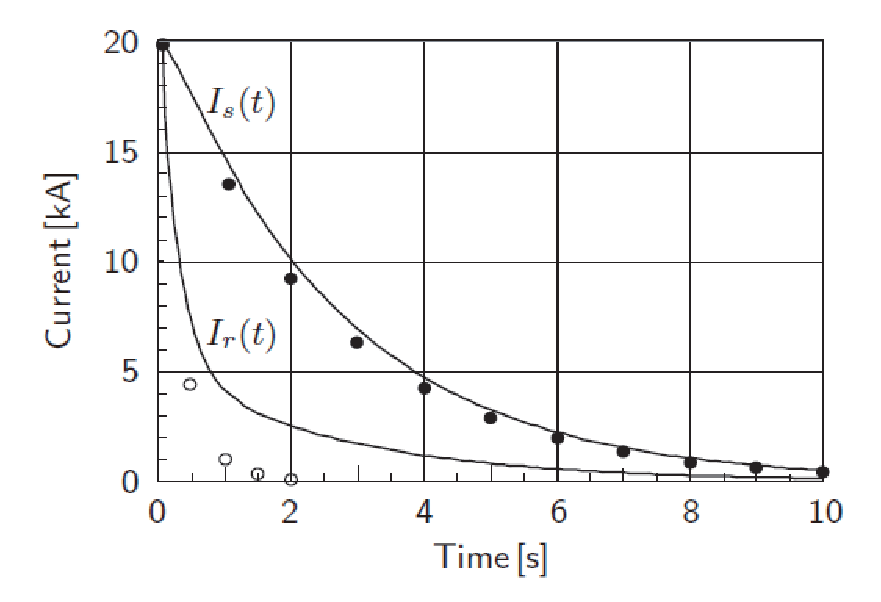
\includegraphics[scale=0.5]{chpt9/figs/fig9.3.eps}
	\caption{方程m.3两式在$M_{sr}=0$的曲线,实心点为$I_s(t)$,空心点为$I_r(t)$。各点列旁边的曲线是$M_{sr}$=0.017 H对应的解。}
\end{figure}

\textbf{n) 耦合效应}\qquad 两磁体显然是感性耦合的---$M_{sr}\neq 0$。
解释图9.3中,为什么$M_{sr}$=0.017 H对应的$I_s(t)$解在$M_{sr}=0$的实心点列上方。

\textbf{解:}我们可以把m.1的第一式写为
\begin{align*}% page552 第1个
L_s\frac{dI_s(t)}{dt}=-R_DI_s(t)-M_{sr}\frac{dI_r(t)}{dt} \tag{n.1}
\end{align*}
因为$dI_r(t)/dt<0$,方程n.1中的$-M_{sr}dI_r(t)/dt$为正,
从而令$|dI_r(t)/dt|$在$M_{sr}\neq 0$时要比在$M_{sr}=0$时小。
也即,$M_{sr}\neq 0$时的$I_s(t)$要比$M_{sr}=0$时衰减的更慢。
但是,因为$k_{sr}$并不很大,假定$M_{sr}=0$的快速解偏离并不大,至少对$I_s(t)$是如此。

\textbf{o) 有效衰减时间常数}\qquad 如上文n)中所述,当将两个磁体之间的电感耦合考虑进来后,
$I_s(t)$和$I_r(t)$相比m)中的不耦合系统衰减的更慢。
假设超导磁体在20 kA时储存的总磁能是55.4 MJ(按e)的计算)全部耗散于电阻$R_D$,
耦合系统中的$I_s(t)$使用“有效”时间常数$\tau_{eff}$表示,计算$\tau_{eff}$。

\textbf{解:}超导磁体的总磁能耗散于$R_D$,有:
\begin{align*}% page552 第2个
E_s=R_D\int_{0}^{\infty}I_s^2(t)dt \tag{o.1a}
\end{align*}
因为$I_s(t)=I_o e^{-t/\tau_{eff}}$,上式成为:
\begin{align*}% page552 第3个
E_s=R_D\int_{0}^{\infty}I_{o}^2e^{-2t/\tau_{eff}}dt=\frac{R_DI_o^2\tau_{eff}}{2} \tag{o.1b}
\end{align*}
解出上式的$\tau_{eff}$,有:
\begin{align*}% page552 第4个
\tau_{eff}=\frac{2E_s}{R_DI_o^2}=\frac{2(55.4\times10^6\ \mathrm{J})}{(0.1\ \mathrm{\Omega})(2\times10^4\ \mathrm{A})^2}=2.77\ \mathrm{s}
\end{align*}
可见,计算值比不耦合系统的计算值2.6 s略大$\sim6\%$。

\textbf{p) 磁滞损耗}\qquad 磁体从0到$B_m$励磁过程中,各超导丝中产生磁滞损耗。
估计一根直径为$d_f$=42 $\mu$m,位于CIC导体最内层之中的Nb2Sn细丝的空间平均磁滞能量密度$e_{hy1}$,
磁体缓慢通电流到20 kA,对应磁场为$B_m$=14 T。
从方程7.23a着手,该方程适用于存在传输电流下的Bean板(案例4i):
\begin{align*}% page553 第1个
e_{hy}=\frac{1}{2}\mu_oH_pH_m(1+i)^2\     \ [H_m\geq H_p(1-i)] \tag{7.23a}
\end{align*}
因为我们处理的导线假定为圆截面,直径为$d_f$,使用$H_p=(8/3\pi)J_c(d_f/2)$,该式
适用于垂直磁场下的导线(方程5.29b)。
接下来,因为$I_t$自0始,到20 kA止,远小于将近40 kA的$I_c$,令$(1+i)^2\simeq 1$可化简方程。
决定$H_p$的$J_c$在0和14 T之间宽幅变动。
也即,我们必须从$\mu_o H_m=B_m=0$到$B_m$=14 T对方程7.23a积分,
得到20 kA下最内层内的平均场:
\begin{align*}% page553 第2个
e_{hy1}\simeq\frac{2d_f}{3\pi}\int_{0}^{B_m}J_c(B,t,\epsilon)dB \tag{p.1}
\end{align*}
这里,$J_c(B,t,\epsilon)$是Nb3Sn的临界电流密度,其依赖性不仅考虑了B和T,还包括了
应力$\epsilon$。这是因为磁体在充磁和退磁过程中,作用于每一根导体丝上的应力是变化的。
对T的依赖也是很重要的,因为如果磁体充磁或退磁的过程不是足够缓慢从而导体可以在
可以忽略的温升下将热传给制冷剂,导体的温度降升高。
通常,p.1以闭式解积分将非常复杂。

不过,我们将在这里使用闭式解,通过:1) 以足够缓慢的速度改变磁场,维持导体温度为4.5 K;
2) 忽略应力对$J_c$的效应。对处于磁体中平面和最内层的Nb3Sn复合导体丝,我们可以使用
平均电流密度$\tilde{J}_c(B,4.5K0)$:
\begin{align*}% page553 第3个
\tilde{J}_c(B,4.5K,\epsilon=0)=\tilde{J}_c(0,4.5K)\frac{b_o}{b_o+B} \tag{p.2}
\end{align*}
式中,$\tilde{J}_c(0,4.5K)=42\times 10^9\ \mathrm{ A/m^2}$,
$b_o$=1 T。
方程p.2是Nb3Sn在4.5 K和$\epsilon=0$下的$\tilde{J}_c(B,T,\epsilon)$的粗略近似。

\textbf{解:}使用p.2,我们首先积分:
\begin{align*}% page553 第4个
\int_{0}^{B_m}\tilde{J}_c(B,4.5\ \mathrm{K})dB&=\tilde{J}(0,4.5\ \mathrm{K})b_o\int_{0}^{B_m}\frac{dB}{b_o+B}=\tilde{J}_c(0,4.5\ \mathrm{K})b_o\ln(\frac{b_o+B_m}{b_o})\\
&=(42\times10^9\ \mathrm{J/m^2})(1\ \mathrm{T})\ln15=113.7\times10^9\ \mathrm{J/m^4}
\end{align*}
将上式结果代入p.1,有:
\begin{align*}% page553 第6个
e_{hy1}\simeq\frac{2(42\times10^{-6}\ \mathrm{m})}{3\pi}(113.7\times10^9\ \mathrm{J/m^4})\simeq1014\ \mathrm{kJ/m^3}
\end{align*}
使用GRANDLF,Gavrilin根据p.1得到$e_{hy1}=1039\ \mathrm{kJ/m^3}$;
在我们的简化模型下,他得到$1122\ \mathrm{kJ/m^3}$---
该值略大因为$J_c(B,4.5\ \mathrm{K},\epsilon=0)>J_c(B,T>4.5\ \mathrm{K},\epsilon>0)$[9.2]。

\textbf{q) 充电速率 vs. 氦温升}\qquad 流体力学上看,该磁体的各层是并联的。
假定进入制冷工质的唯一热源是空间平均分布的磁滞损耗,计算磁体从0到20 kA
最大的恒电流充电速度$(dI_s/dt)_{mx}$,在该速度下,氦质量流量若为5 g/s,
氦的时间平均温升极限为$\Delta\tilde{T}_{he}\simeq 4.0$ K($=\tilde{T}_{cs}-T_{op}$)。
这里,$\tilde{T}_{cs}$是时间平均的电流分享温度,在$I_{op}$=0时,$T_{cs}$=10.3 K;
在$I_{op}$=20 kA时,$T_{cs}$=6.7 K:$\tilde{T}_{cs}$=8.5 K。
此处计算使用p)中在恒定温度下得到的$e_{hy}=1014\ \mathrm{kJ/m^3}$。

氦在4.5 K和3.5 atm下的物性如下:定压比热$C_{he}$=4.28 J/gK;
密度$\rho_{he}=0.132\ \mathrm{g/cm^3}$,且认为其在最内层与温度和压力无关。
首先,证明在最内层释放的磁滞损耗总能量$E_{hy1}$为3.5 kJ。

\textbf{解:}最内层释放的磁滞损耗总能量为:
\begin{align*}% page554 第1个
E_{hy1}=e_{hy}(A_{sc}+A_{\bar{m}})\ell_1
\end{align*}
式中,$(A_{sc}+A_{\bar{m}})=40.2\ \mathrm{ mm^2}$,$\ell_1$是最内层的导体总长度。
我们有$\ell_1\simeq 2\pi(a_1+w)(42)$,其中,$a_1$是绕组的内径,$w$是槽的径向深度,
42是每层的匝数---上述数据可从表9.1查得。
从图9.1和表9.1我们知道,磁体绕组的径向尺度$a_2-a_1$是305.1 mm,
包括18层CIC导体:$w$=(305.1 mm)/18$\simeq$17 mm。于是:
\begin{align*}% page554 第2个
\ell_1\simeq 2\pi(0.305\ \mathrm{m}+0.017\ \mathrm{m})42\simeq 85\ \mathrm{m}
\end{align*}
\begin{align*}% page554 第3个
E_{hy1}=(1014\times 10^3\ \mathrm{J/m^3})(40.2\times 10^{-6}\ \mathrm{m^2})(85\ \mathrm{m})\simeq 3.5\ \mathrm{kJ}
\end{align*}

在流量$\.{m}_{he}$=5 g/s下,氦的焓在最内层入口到出口的时间平均变化率$dH_{he}/dt$为:
\begin{align*}% page554 第4个
\frac{dH_{he}}{dt}&=C_{he}m_{he}\Delta\tilde{T}_{he}\\
&=(4.28\ \mathrm{J/gK})(5\ \mathrm{g/s})(4.0\ \mathrm{K})\simeq 86\ \mathrm{W}
\end{align*}
也即,在时间平均温升为4.0 K时,最内层的氦的冷却功率为86 W。
该冷却功率必须与最大耗散率$P_{{hy1}_{mx}}$相匹配:
\begin{align*}% page554 第5个
 P_{hy1_{mx}}\simeq\frac{E_{hy1}}{\Delta t_{mn}}=86\ \mathrm{W} \tag{q.1}
\end{align*}
在方程q.1中解出$\Delta t_{mn}$,我们得到:
\begin{align*}% page554 第7个
\Delta t{mn}=\frac{E_{hy1}}{P_{hy1_{mx}}}\simeq\frac{3.5\ \mathrm{kJ}}{86\ \mathrm{W}}\simeq 41\ \mathrm{s}
\end{align*}
于是:
\begin{align*}% page554 第8个
(\frac{dI_s}{dt})_{mx}=\frac{\Delta I_s}{\Delta t_{mn}}\simeq\frac{20\times 10^3\ \mathrm{A}}{41\ \mathrm{s}}\simeq 490\ \mathrm{A/s}
\end{align*}

这样,额定充电速度400 A/s可以保证导体低于其电流分享温度,该温度在$I_{op}=0$时
为10.3 K,在$I_{op}=20$ kA时为6.7 K。

\textbf{r) 耦合损耗}\qquad 使用方程7.36和7.39c (表7.8),计算耦合耗散能量密度$e_{cp}$。
计算条件为:导体细丝直径$D_{mf}$=0.6 mm,$\ell_p$=10 mm,
以很定充电速率400 A/s线性或$\tau_m$=50 s(如图7.18的三角形场激励)
将磁体由0充电至20 kA($B_m$=14 T)。
对于本Nb3Sn细丝,$\tau_{cp}$=30 ms[9.2]。

\textbf{解:}在$\tau_m\gg \tau_{cp}$下,三角波激励下的时间平均$e_{cp}$由7.36和7.39c的组合形式给出:
\begin{align*}% page555 第1个
e_{cp}=2\mu_oH_{m}^2[1+\frac{1}{4}(\frac{\pi D_{mf}}{\ell_p})^2]\Gamma \tag{7.36}
\end{align*}
\begin{align*}% page555 第2个
\Gamma\simeq\frac{4\tau_{cp}}{\tau_m}\   \  (\tau_m\gg \tau_{cp}) \tag{7.39c}
\end{align*}
方程7.36中,$(\pi D_{mf}/\ell_p)^2\ll 1$,$H_m=B_m/\mu_o$;
充电时间周期仅包括整个三角波的1/2(图7.18),
所以方程7.36中必须加入因子1/2。这样,$e_{cp}$成为:
\begin{align*}% page555 第3个
e_{cp}&\simeq\frac{1}{2}(2\frac{B_m^2}{\mu_o})\Gamma\\
&=\frac{4B_m^2\tau_{cp}}{\mu_o\tau_m} \tag{r.1}
\end{align*}

代入$B_m$=14 T,$\tau_{cp}$=30 ms以及$\tau_m$=50 s,我们得到:
\begin{align*}% page555 第5个
e_{cp}=\frac{4(14\ \mathrm{T})^2(30\times 10^{-3}\ \mathrm{s})}{(4\pi\times 10^{-7}\ \mathrm{T})(50\ \mathrm{s})}\simeq 357\ \mathrm{kJ/m^3}
\end{align*}

可见,耦合损耗约为磁滞损耗的$\sim 1/3$。

\textbf{s) 热点温度}\qquad 假定$t=0$时,超导磁体中检测到失超,断路器无时延打开---
即在$t=0$时刻打开。假定超导磁体中的电流$I_s(t)$以指数衰减,等效衰减常数$\tau_{eff}$=2.77 s
(如o)中所得)。同时假定初始失超点---“热点”---由焦耳热绝热加热。
计算热点的最终温度$T_f$。
同时假设,仅由CIC导体---超导体、非基底金属、基底(铜,RRR=100)---吸收焦耳热,
铜的热容量可用来代表全部导体的热容量。

\textbf{解:}根据方程8.16a,我们有:
\begin{align*}% page556 第1个
Z(T_f,T_i)=(\frac{A_m}{A_{cd}})\int_{0}^{\infty}J_{m_o}^2e^{-2t/\tau_{dg}}dt=(\frac{A_m}{A_{cd}})J_{m_o}^2\times\frac{1}{2}\tau_{dg} \tag{8.16a}
\end{align*}

将表9.1中的参数代入8.16a,$A_m=57.4\ \mathrm{mm^2}$;
$A_{cd}=A_m+A_{sc}+A_{\bar{m}}=97.6\ \mathrm{ mm^2}$;
$J_{m_{op}}=I_{op}/A_m=20000/57.4\times 10^{-6}=3.48\times 10^8\ \mathrm{ A/m^2}$;
将$\tau_{dg}=\tau_{eff}$=2.77 s代入s.1,解铜的$Z_{cu}(T_f,T_i)$,$Z(T_f,T_i)$:
\begin{align*}% page556 第2个
Z_{cu}(T_f,T_i)&=(\frac{57.4\times 10^{-6}\ \mathrm{m^2}}{97.6\times 10^{-6}\ \mathrm{m^2}})(3.48\times 10^8\ \mathrm{A/m^2})^2(\frac{2.77\ \mathrm{s}}{2})\\
&\simeq 9.9\times 10^{16}\ \mathrm{A^2s/m^4}
\end{align*}

从图8.2,我们找到$Z_{cu}(T_f,T_i=4.5\ \mathrm{K})=9.9\times 10^{16}\ \mathrm{A^2 s/m^4}$对应
铜(RRR=100)的$T_f\simeq 125$ K。

\textbf{t) 起始延时}\qquad 一个更贴近实际的场景应考虑从$t=0$热点出现到断路器实际打开的延时$\tau_{dl}$。
这是因为热点电压升高到触发断路器打开所需的水平需要一定时间。
假设这个期间$t_d$内,超导磁体的电流保持20 kA,估算热点最终温度$T_f$。除$\tau_{dl}$=0.5 s外,
条件假设同s)。

\textbf{解:}使用方程8.66b,并使用$\tau_{eff}$代替$\tau_{dg}$,有:
\begin{align*}% page557 第1个
Z(T_f,T_i)&=(\frac{A_m}{A_{cd}})(\tau_{dl}+\frac{1}{2}\tau_{eff})J_{m_{op}}^2\\
&\simeq 13.5\times 10^{16}\ \mathrm{A^2s/m^4}
\end{align*}

从图8.2,我们找到$Z_{cu}(T_f,T_i=4.5\ \mathrm{K})=13.5\times 10^{16}\ \mathrm{A^2 s/m^4}$
对应铜(RRR=100)的$T_f\simeq 225$ K,这几乎是可接受的热点温度的极限了。
尽管实际中由于制冷工质的冷却,$T_f$应能<225 K,但出于谨慎考虑,磁体产生热点后断路器应
确保在0.5 s内打开。
这意味着热点产生后,必须在远小于0.5 s的时间内将之检测到。

图9.4给出了温度(实线)和压力(虚线)与时间的关系图。该图由Gavrilin[9.2]制作,他使用GANDALF
计算了类似于s)的案例,他的计算中除了使用了$I_s(t)$的准确解,还考虑了氦的冷却效果和交流损耗。
大体上说,由于氦的冷却,热点温度$T_f$仅上升到$\sim$95 K,而不是s)中在绝热和$\tau_{dl}=0$
条件下计算的125 K。
分析还表明,通道内氦的压力峰值达到了23.5 atm。
\begin{figure}[htbp]
	\centering
	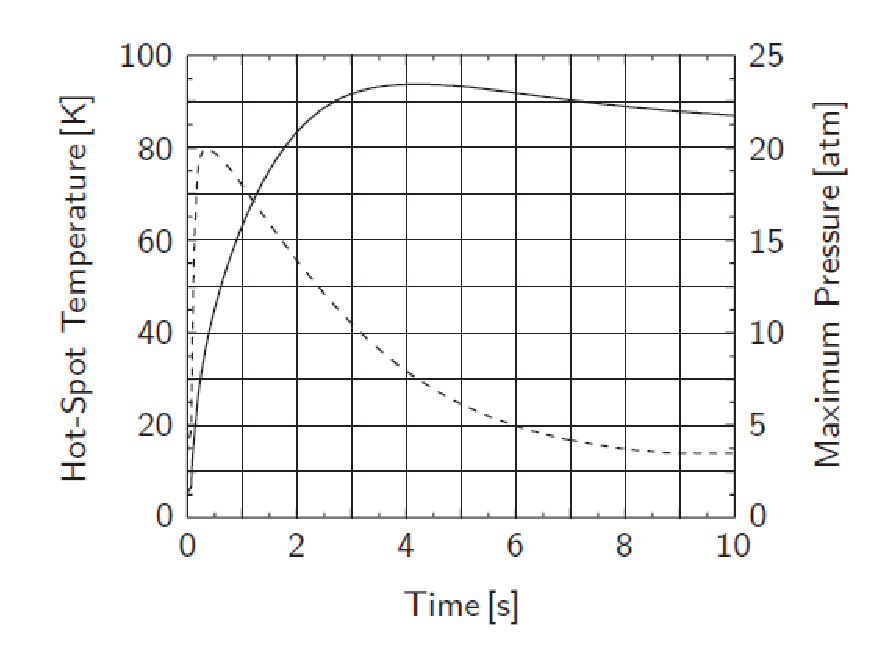
\includegraphics[scale=0.6]{chpt9/figs/fig9.4.eps}
	\caption{温度(实线,左y轴)和压力(虚线,右y轴)与时间的关系。}
\end{figure}

表9.2.。。。。。。。。。。。。。。。。。。。。


\textbf{u) 故障模式轴向力}\qquad SCH磁体的一个可能故障模式就在额定运行电流20 kA下,
5个电阻型插入线圈(图9.1)的各线圈的一半损坏(最恶劣情景)而形成电气短接,剩余一半继续工作产生磁场。
各线圈的上半部分短接时,各线圈的轴向场中心下移$b/2$;
对线圈5(最外侧),由图9.1可见,该值为$151\frac{1}{4}$ mm。
表9.2给出了5线圈电阻型插入磁体的关键参数[9.3]。

当这种情况发生后,超导磁体承受向下的轴向力,该力与电阻型磁体的承受向上力一致。
从图9.1我们可以看到,超导磁体承受的最大力来自线圈5,尽管其中心场是最小的。主要原因是:
1) 线圈5最大;2)它与超导磁体耦合最紧密。
参照下面给出的逐步的“简单”但“理由充分”的步骤,粗略计算线圈5和4对超导磁体的力。
这里的目标是让一个设计小组的非专家获得大致认知,组内的专家则会使用程序计算得到“精确”的数值。

3.5节,我们讨论了计算“简单”螺管线圈组合,特别是“环”线圈,薄壁线圈等的解析方法。
这些组合中,最简单的是两个环形线圈之间的力的计算(图3.5):
线圈A,直径$a_A$,总匝数$N_A$,电流$I_A$;线圈B,直径$a_B$,总匝数$N_B$,电流$I_B$。

\textbf{逐步过程}

过程包括两步。
\begin{description}
	\item[第一步] 将各线圈建模为环形线圈,使其产生和原始线圈相同的中心场。计算环形线圈在运行电流
	20 kA下的总匝数$N$。尽管超导磁体和电阻型线圈建模为薄壁螺管线圈更准确(图3.7),
	但相应的轴向力表达式更复杂,对评估大致情况显得不必要。
\item[第二步] 使用方程3.34计算两个环线圈之间的轴向力:首先是超导环线圈(线圈A)和电阻型环线圈5(线圈B)
之间的力;接下来计算超导环线圈(线圈A)和电阻型线圈4(线圈B)之间的力。
\end{description}

\textbf{两个环线圈之间的轴向力:复习}

对两个轴向距离$\rho$的环形线圈A和线圈B,两线圈之间的轴向力$F_{zA}(\rho)$为:
\begin{align*}% page559 第1个
F_{AZ}(\rho)=&\frac{\mu_o}{2}(N_AI_A)(N_BI_B)\frac{\rho\sqrt{(a_A+a_B)^2+\rho^2}}{(a_A-a_B)^2+\rho^2}\\
&\times\{k^2K(k)+(k^2-2)[K(k)-E(k)]\} \tag{3.34}
\end{align*}
$K(k)$和$E(k)$分别是第一类和第二类完全椭圆积分。
该系统椭圆积分的模量$k$为:
\begin{align*}% page559 第2个
k^2=\frac{4a_Aa_B}{(a_A+a_B)^2+\rho^2} \tag{3.36}
\end{align*}

\textbf{解:}使用方程3.111a给出的场表达式计算超导环形线圈A的匝数$N_A$:
\begin{align*}% page559 第3个
B_z(0,0)=\frac{\mu_oNI}{2a_1} \tag{3.111a}
\end{align*}
这里,$N=N_A,I=I_A, a_1=a_A$。
超导线圈的$a_A$的一个合适的值时平均绕组半径(表9.1):$a_A\simeq$458 mm。
于是,代入$B_Z(0,0)$=14.52 T和$I_A$=20 kA,我们有:
\begin{align*}% page559 第4个
N_A=\frac{2a_AB_Z(0,0)}{\mu_oI_A}=\frac{2(0.458\ \mathrm{m})(14.52\ \mathrm{T})}{(4\pi\times 10^{-7}\ \mathrm{H/m})(2\times 10^4\ \mathrm{A})}=529
\end{align*}

我们注意到$N_A$比磁体实际的匝数756小,这是由于产生相同的中心场,环形线圈要比
各匝分布于很大的绕组截面上的实际磁体效率高。

将线圈5建模为环形线圈B需要更加的小心:中心场3.72 T不能直接使用,因为这是线圈5在故障前
产生的中心场。现在,轴向距离$2b$折半了,于是,我们必须首先计算线圈5在$\beta'=\beta/2$
时产生的中心场。
对于Bitter磁体,场因子$[F(\alpha,\beta)]_B$由方程3.115b给出:
\begin{align*}% page559 第5个
[F(\alpha,\beta)]_B=\ln(\alpha\frac{\beta+\sqrt{1+\beta^2}}{\beta+\sqrt{\alpha^2+\beta^2}}) \tag{3.115b}
\end{align*}

因为损坏线圈中的“健康”的一半线圈的参数不变,新的中心场$[B_Z'(0,0)]_B$
可以由原中心场$[B_Z(0,0)]_B$给出:
\begin{align*}% page559 第6个
\frac{[B_Z'(0,0)]_B}{[B_Z(0,0)]_B}
=\frac{[F(\alpha,\beta')]_B}{[F(\alpha,\beta)]_B}
=\frac{\ln(\alpha\frac{\beta'+\sqrt{1+\beta'^2}}{\beta'+\sqrt{\alpha^2+\beta'2}})}{\ln(\alpha\frac{\beta+\sqrt{1+\beta^2}}{\beta+\sqrt{\alpha^2+\beta^2}})} \tag{u.1}
\end{align*}

将线圈5的以下值代入方程u.1:$[B_z(0,0)]_B=3.72$ T,$\alpha\simeq$1.44(=500.0 mm/347.8 mm),
$\beta\simeq$1.74(=605 mm/347.8 mm),$\beta'=\beta/2\simeq$1.74/2=0.87。
解出$[B'_z(0,0)]_B$,我们得$[B'_z(0,0)]_B$=2.66 T。

线圈5'的$a_B$一个合理值是其几何平均值$a_B=\sqrt{a_1 a_2}$=208.5 mm而不是算术平均值
$(a_1+a_2)/2$=212.0 mm。这是因为Bitter线圈中电流密度是不均匀的,而是随$\propto 1/r$变动(方程3.114)。
为了简化,我们取$a_B$=174 mm。这样,代入$[B'_z(0,0)]_B$=2.66 T和$I_B=$20 kA:
\begin{align*}% page560 第1个
N_B=\frac{2(0.174\ \mathrm{m})(2.66\ \mathrm{T})}{(4\pi\times 10^{-7}\ \mathrm{H/m})(2\times 10^4\ \mathrm{A})}\simeq 37
\end{align*}
代入$a_A$=0.458 m,$a_B$=0.174 m,$a_A+a_B$=0.632 m和$\rho=$0.151 m(线圈5原始值的1/4),
首先计算出模量$k$:
\begin{align*}% page560 第2个
k^2&=\frac{4a_Aa_B}{(a_A+a_B)^2+\rho^2}\\ \tag{3.36}
&=\frac{4(0.458\ \mathrm{m})(0.174\ \mathrm{m})}{(0.632\ \mathrm{m})^2+(0.151\ \mathrm{m})^2}\\
&\simeq 0.7550\ \ (k\simeq 0.8689)
\end{align*}
向方程3.34中代入$K(0.8689)=2.1655, E(0.8689)=1.2079, a_A-a_B=0.284$ m和其他参数,
我们得到线圈B(线圈5的一半)施于线圈A(超导磁体)的力$F_{zA}(\rho=151\ \mathrm{mm})$为:
\begin{align*}% page560 第5个
F_{zA}(151\ \mathrm{mm})=&\frac{4\pi\times10^{-7}\ \mathrm{H/m}}{2}(529)(2\times 10^4\ \mathrm{A})(37)(2\times 10^4\ \mathrm{A})\\
&\times[\frac{(0.151\ \mathrm{m}\sqrt{(0.632\ \mathrm{m})^2+(0.151 \ \mathrm{m})^2})}{(0.284\ \mathrm{m})^2+(0.151\ \mathrm{m})^2}\\
&\times\{0.7550(2.1655)+(0.7550-2)(2.1655-1.2079)\}]\\
=&(4.92\ \mathrm{MN})\times[0.948\times 0.443]=2.06\ \mathrm{MN}
\end{align*}

为了计算线圈B(线圈4的一半)施于线圈A的力,我们有线圈B的以下新参数:
$\alpha=1.41;\beta=1.46;\beta'=0.73;B'_z(0,0)$=2.96 T;$N_B\simeq 28; a_B=0.121$ m。
代入$\rho$=0.088 m; $a_A+a_B$=0.579 m; $a_A-a_B$=0.337 m,我们有:
$k^2\simeq 0.6463(k\simeq 0.8039)$,对应给出的$K(0.8039)\simeq 2.0030, E(0.8039)\simeq 1.2728$。
将这些值代入方程3.34,我们得到$F_{zA}(88\ \mathrm{mm})=0.49$ MN。
该值比线圈5初始所施的力的1/4,意味着线圈1-3的贡献可以忽略。

采用程序计算的线圈1-5的合力是1.9 MN[9.3]。
我们的基于简化模型的方法需要用计算器按上一段时间,最终给出的结果似乎2.06 MN(仅来自线圈5),
这个值作为估算来讲已经够好。

\textbf{磁场屏蔽}

因为磁体越大(尺寸、场强或两者都大),它的边缘场延伸的范围越大,故“大”磁体通常需要屏蔽。
主动屏蔽使用电磁体(屏蔽线圈);被动屏蔽使用铁磁结构(钢壳)。
主动屏蔽为保证其他设计参数,应离主磁体尽可能的远,因为它会弱化磁场;
被动屏蔽通常增加磁场。
高场(>1 T)MRI和多数NMR磁体如今都是主动屏蔽、被动屏蔽或两者兼容屏蔽的。

如开始所述,SCH磁体与实验所用空间相邻。为了减少磁体对旁边的实验的磁场干扰,
SCH磁体系统需要一个屏蔽线圈,如图9.5 SCH磁体截面示意图的右侧所示。
有一个很大的室温孔的电阻性磁体,相比超导主磁体来说贡献了很小的边缘场,在图中忽略未画出。
图9.5的左侧给出了一个钢壳,用于被动屏蔽---这是屏蔽超导主磁体的另一种方法。

如图9.5所示,主动屏蔽线圈(本磁体首创[9.1])实际上是由两个子线圈构成,一个放置在中平面上方,另一个在下方;
这里两个子线圈都被建模为环形线圈。
钢壳是圆柱形的,在这里的分析中被建模为周向将主磁体完全围住。两个元件的重要方面此处都将进行研究。

\begin{figure}[htbp]
	\centering
	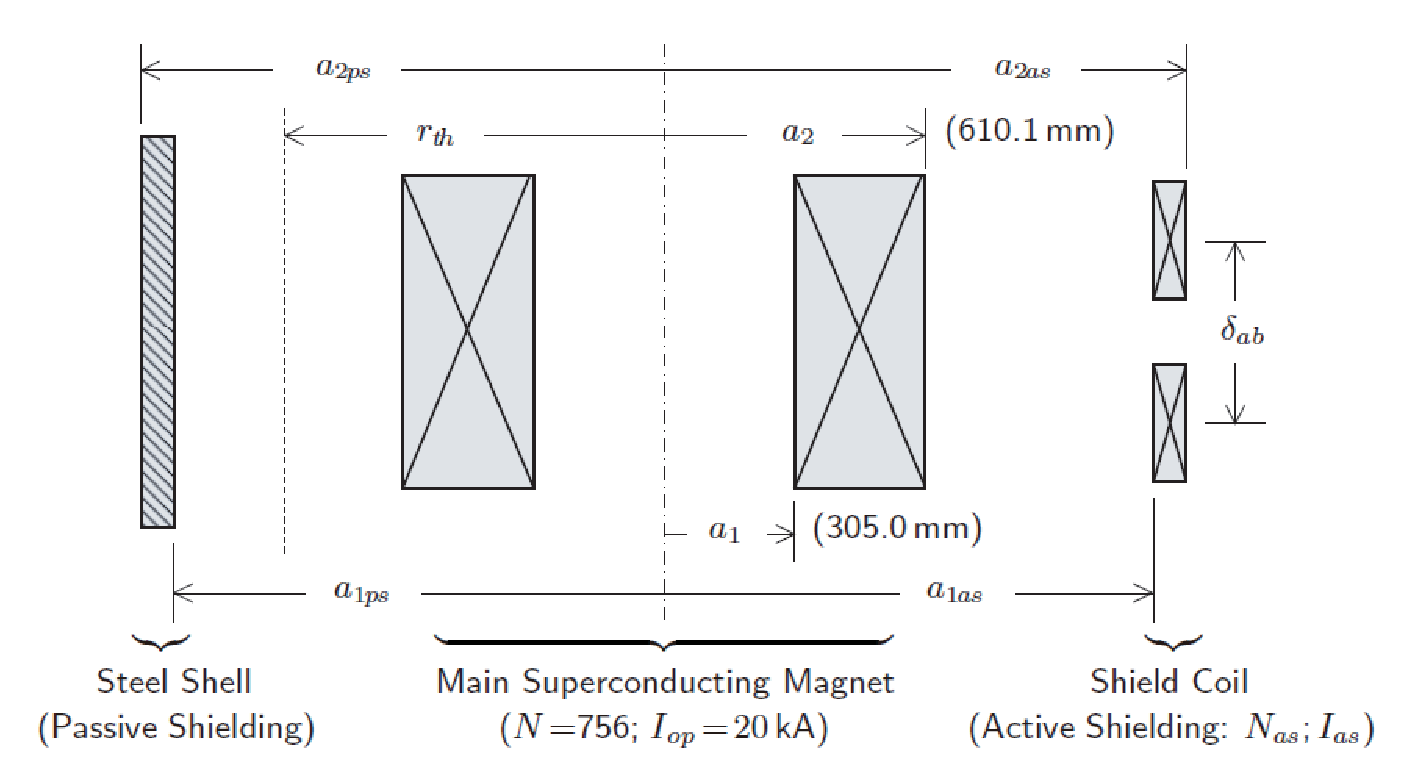
\includegraphics[scale=0.6]{chpt9/figs/fig9.5.eps}
	\caption{主磁体使用屏蔽线圈(主动屏蔽)或钢壳9(被动屏蔽)的截面图。主动屏蔽线圈由两个子线圈组成,分别在
		中平面的上方和下方。}
\end{figure}

\textbf{v) 主动屏蔽线圈---匝数}\qquad 将两个用于磁屏蔽的子线圈建模为\textit{单}屏蔽线圈。
然后,将超导主磁体线圈和上述屏蔽线圈转换为偶极子。
现在,估算这个模型屏蔽线圈的总匝数,令其磁极矩与主磁体的极矩匹配。
屏蔽线圈和运行于20 kA的主磁体串联,但极性相反。

\textbf{解:} 远离螺管磁体中心的磁场$\vec{H}_f$可以建模为偶极子(问题3.1):
\begin{align*}% page562 第1个
\vec{H}_f=H_0(\frac{R_e}{r})^3(\cos\theta{\vec{\imath}_r}+\frac{1}{2}\sin\theta\vec{\imath}_\theta) \tag{3.163}
\end{align*}
$R_e$是偶极子的半径。
对一个安匝$NI$均匀分布的螺管,乘积$H_0 R_e^3$由下式给出:
\begin{align*}% page562 第2个
H_0R_e^3=\frac{1}{6}(a_1^2+a_2^2+a_1a_2)NI \tag{3.165}
\end{align*}
式中,$a_1$和$a_2$分别是磁体绕组的内外半径。
因为$\vec{H}_f\propto (R_e/r)^3$以及$H_0 R_e^3\propto a_1^2$,
这里,我们实际上可以忽略电阻性插入磁体---线圈5的$a_1$=173.9 mm,
超导磁体的$a_1$=305.0 mm。
对主超导磁体和屏蔽线圈(下标$as$)分别应用方程3.163和3.165,有:
\begin{align*}% page562 第3个
a_1^2(1+\alpha^2+\alpha)NI_{op}=a_{1as}^2(1+\alpha_{as}^2+\alpha_{as})N_{as}I_{as} \tag{v.1}
\end{align*}
其中,$\alpha_{as}=a_{2as}/a_{1as}$。代入$I_{as}=I_{op}$,从v.1中解出$N_{as}$:
\begin{align*}% page562 第4个
N_{as}=(\frac{a_1}{a_{1as}})^2(\frac{1+\alpha^2+\alpha}{1+\alpha_{as}^2+\alpha_{as}})N \tag{v.2}
\end{align*}
将$a_1$=0.305 m,$a_{1as}$=1.203 m,$\alpha=2.00$,$\alpha_{as}$=1.04和$N$=756代入
v.2,$N_{as}$成为:
\begin{align*}% page562 第5个
N_{as}=(\frac{0.305\ \mathrm{m}}{1.203\ \mathrm{m}})^2(\frac{1+4+2}{1+0.8+1.04})(756)\simeq 109
\end{align*}

屏蔽线圈的实际匝数似乎78[9.4],并且是由两个如图9.5所示的子线圈组成的。
轴向绕匝的位移未引起磁矩衰减;若匝数轴向展开,仅磁场降低。

\textbf{w) 主动屏蔽线圈对中心场的减弱}\qquad 前文提及,主动屏蔽线圈产生于超导主磁体反向的磁场。
计算主动屏蔽线圈在中心的轴向场$B_z^{as}(0,0)$。
屏蔽线圈使用以下参数:$a_{1as}$=1.203 m;$a_{2as}$=1.250 m;
$b_{as}$=0.471 m(实际系统中,主动屏蔽线圈由两个稍短的子线圈构成,两者各据中平面有一个间隙[9.4]);
$N_{as}$=78;和$I_{as}$=20 kA。

\textbf{解:}磁场的计算是方程3.110的直接应用:
\begin{align*}% page563 第1个
B_z(0,0)=\frac{\mu_oNI}{2a_1(\alpha-1)}\ln(\frac{\alpha+\sqrt{\alpha^2+\beta^2}}{1+\sqrt{1+\beta}}) \tag{3.110}
\end{align*}
代入$N\rightarrow N_{as}=78$,$I\rightarrow I_{as}$=20 kA,$\alpha\rightarrow \alpha_{as}$=1.04,
$\beta\rightarrow \beta_{as}=0.392$以及$a_1\rightarrow a_{1as}=1.203$,
$B_z^{as}(0,0)$成为:
\begin{align*}% page563 第2个
B_z^{as}(0,0)&=\frac{(4\pi\times 10^{-7}\ \mathrm{H/m})(78)(20\times 10^3\ \mathrm{A})}{(2.406\ \mathrm{m})(1.04-1)}\ln(\frac{1.04+\sqrt{(1.04)^2+(0.392)^2}}{1+\sqrt{1_(0.92)^2}})
&\simeq 0.75\ \mathrm{T}
\end{align*}

因为若无主动屏蔽线圈,20 kA的超导主磁体的中心场是14.52 T(Q/A 9.1的问题b)计算所得),
主动线圈将之降低了0.75 T,约为5\%。总的来看,已经不能忽视。

\textbf{x1) 主动屏蔽线圈---作用力:1}\qquad 如果屏蔽线圈建模为单线圈,那么它和主磁体之间不会有
净作用力。在原始系统中,屏蔽线圈被分为两个子线圈。
此时,作为整体的屏蔽线圈和主磁体之间仍无净作用力,
但是各子线圈与主磁体之间均存在作用力。
这里我们将主磁体和其中一个子线圈均建模为“环线圈”,计算其作用力的大致幅值。
取$\rho$=0.227 m(中心对中心距离)。
由于图9.5中的$\delta_{ab}=2\rho$,$\delta_{ab}$=0.554 m。

\textbf{解:}在前文t)中,主磁体已被建模为环形线圈:$N_A$=529;$a_A\simeq$458 mm。
类似的,我们可以将其中的一个子线圈建模为环线圈,使其产生中心场0.375 T(0.75 T的一半,
尽管两者是垂直放置的):
$a_B$=1.227 m($a_{1as}$和$a_{2as}$的平均值),$N_B$为:
\begin{align*}% page563 第3个
N_B\simeq\frac{(0.375\ \mathrm{T})2(1.227\ \mathrm{})}{(4\pi\times 10^{-7}\ \mathrm{H/m})(20\times 10^3\ \mathrm{A})}\simeq 37
\end{align*}

由于各子线圈的$\alpha=1.04$和很小的$\beta$表明它们非常接近环形线圈($\alpha=1,\beta=0$),
所以“有效匝数”37与实际匝数39如此接近并不令人惊讶。
首先,我们使用t)节用到的方程3.36计算模量常数$k$:
\begin{align*}% page563 第4个
k^2&=\frac{4a_Aa_B}{(a_A+a_B)^2+\rho^2}\\ \tag{3.36}
&=\frac{4(0.458\ \mathrm{m})(1.227\ \mathrm{m})}{(0.458\ \mathrm{m+1.227\ \mathrm{m}})^2+(0.227\ \mathrm{m})^2}\simeq 0.7709\   \ (k\simeq 0.8780)
\end{align*}

两个环线圈之间的作用力由3.34给出:
\begin{align*}% page564 第1个
F_{ZA}(\rho)=&\frac{\mu_o}{2}(N_AI_A)(N_BI_B)\frac{\rho\sqrt{(a_A+a_B)^2+\rho^2}}{(a_A-a_B)^2+\rho^2}\\
&\times\{k^2K(k)+(k^2-2)[K(k)-E(k)]\} \tag{3.34}
\end{align*}
代入$K(0.8780)=2.1957,E(0.8780)=1.1977,a_A+a_B=$1.685 m, $a_A-a_B=$-0.769 m,
我们得到线圈B(上方子线圈)对线圈A(主磁体)的力$F_{ZA}(\rho=0.227\ \mathrm{m})$:
\begin{align*}% page564 第2个
F_{ZA}(0.277\ \mathrm{m})=&\frac{4\pi\times 10^{-7}\ \mathrm{H/m}}{2}(529)(2\times 10^4\  \mathrm{A})(37)(-2\times 10^{4}\ \mathrm{A})\\
&\times \big[\frac{(0.277\ \mathrm{m})\sqrt{(1.685\ \mathrm{m})^2+(0.277\ \mathrm{m}^2)}}{(-0.769\ \mathrm{m})^2+(0.277\ \mathrm{m})^2}\\
&\times\{0.7709(2.1957)+(0.7709-2)(2.1957-1.1977)\}\big]\\
=&-(4.91\ \mathrm{MN})\times(0.7080\times 0.4660)=-1.62\ \mathrm{MN}
\end{align*}

作用在主磁体上的力是负值(向下);同样大小的力作用在中平面上方的屏蔽子线圈,向上;也即,
如果线圈没有约束,它将被推离中平面。
当然,上下两个子线圈对主磁体的合力为零。

\textbf{x2) 主动屏蔽线圈---作用力:2}\qquad 这里我们计算两个子线圈之间的引力。将两个线圈建模为
相同的环形线圈,直径1.227 m,匝数37,电流-20 kA。这里$\rho$=0.554 m,等于图9.5中的$\delta_{ab}$。

\textbf{解:}因为环形线圈直径相同($a$),尽管在这里条件$\rho(=0.554)\ll 2a(=2.454)$并不严格满足,
我们仍使用方程3.34在$\rho\ll 2a$条件下的简化版本3.39d。本例中,$N_B I_B=N_A I_A$:
\begin{align*}% page564 第3个
F_{ZA}(\rho)&\simeq\mu_o(N_AI_A)(N_BI_B)(\frac{a}{\rho})\\ \tag{3.39d}
&=\mu_o(N_AI_A)^2(\frac{a}{\rho})\\
&=(4\pi10^{-7}\ \mathrm{H/m})[(37)(-2\times 10^4\ \mathrm{A})]^2(\frac{1.227\ \mathrm{m}}{0.554\ \mathrm{m}})\\
&\simeq 1.5\ \mathrm{MN}
\end{align*}

这和用程序[9.3]计算得到的1.6 MN非常吻合。

\textbf{y1) 被动屏蔽壳:1}\qquad 除主动屏蔽外,还可以采用被动屏蔽。被动屏蔽使用铁磁材料,通常
是软铁(见问题2.3和表2.5)来实现。
被动屏蔽的优势主要是费用低,但对于“大型”和“高场”磁体,费用优势就没有了。
另一个经常被忽视的优势是它的“逆向屏蔽”能力,即它还能屏蔽相邻磁体的外围磁场对主磁体的影响。
笨重是被动屏蔽的最大劣势。

这里,我们考虑一个钢制圆柱筒,内半径$a_1\equiv a_{1as}=1.203$ m,高$2b_s=2a_{1as}$(图9.5)。
假定主磁体($N=756;I_{op}$=20 kA)可以建模为偶极矩,其$B_0R_e^3$由方程v.1给出(忽略电阻内插磁体),
估算圆柱筒的外半径$a_{2as}$,使其壁厚度足够保证刚的磁化$\mu_o M_s$在1.25 T时仍有较高的值
$(\mu/\mu_o)_{dif}:(\mu/\mu_o)_{dif}=180$(表2.5中的as-cast钢)。

\textbf{解:}$(\mu/\mu_o)_{dif}=180$时,我们可以将之视为理想的$(\mu/\mu_o)_{dif}=\infty$。
由于主磁体的所有磁通都从磁体室温孔发出,位于$r\ge a_{1as}$的磁通将在上方穿入钢制圆柱筒,并在其下方穿出
返回磁体室温孔。
稍微复杂的是磁体外半径$a_2\simeq0.610$ m与钢制圆柱筒内半径$a_{1ps}=1.203$ m之间的环形空间的磁通线。

因钢的磁阻小于空气,磁通线选择通过钢。这样,$r=a_2$之外的磁通线要么直接垂直进入空气
经$b=0.471$ m到达中平面(表9.1),要么首先径向走过距离$a_{1ps}-a_2=0.593$ m达到钢制
圆柱筒上方,而后垂直“无阻”的进入钢内到达中平面。因为0.471 m<0.593 m,
所以这些磁通不会进入钢内。
根据这个判断,我们可以给出一个半径的阈值$r_{th}$,超过该值,磁通线将改路进入钢圆柱筒内,
该值大概是$a_{1ps}-b=0.732$ m。也即,所有的位于$r_{th}$ m到$r=\infty$之间的磁通线
将进入钢制圆柱筒。于是,中平面上在$r_{th}$ m到$\infty$的总磁通$\Phi(r_{th/\infty,z=0})$和中平面上
通过钢的磁通$\Phi_s(z=0)$分别由下式给出,其中$\alpha=a_2/a_1$:
\begin{align*}% page565 第1个
\Phi(r_{th}/\infty,z=0)=\frac{1}{2}[\frac{\mu_oa_1^2(1+\alpha^2+\alpha)NII_{op}}{6}]\int_{r_{th}}^{\infty}\frac{2\pi r}{r^3}dr \tag{y1.1a}
\end{align*}
\begin{align*}
\Phi_{z}(z=0)=\pi(a_{2ps}^2-a_{1ps}^2)(\mu_oM_s) \tag{y1.1b}
\end{align*}
因为上述两个磁通相等,我们有:
\begin{align*}% page565 第3个
\frac{\mu_oa_1^2(1+\alpha^2+\alpha)NI_{op}}{6r_{th}}=(a_{2ps}^2-a_{1ps}^2)(\mu_oM_s) \tag{y1.2}
\end{align*}
在上式中解出$a_{2ps}$,我们得到:
\begin{align*}% page565 第4个
a_{2ps}=\sqrt{a_{1ps}^2+\frac{\mu_oa_1^2(1+\alpha^2+\alpha)NI_{op}}{6r_{th}(\mu_oM_s)}} \tag{y1.3}
\end{align*}
向y1.3中代入合适的值,计算得:
\begin{align*}% page566 第1个
a_{2ps}&=\sqrt{(1.203\ \mathrm{m})^2+\frac{(4\pi\times 10^{-7}\ \mathrm{H/m})(0.305\ \mathrm{m})^2(7)(756)(20\times 10^3\ \mathrm{A})}{6(0.732\ \mathrm{m})(1.25\ \mathrm{T})}}\\
&=\sqrt{1.447\ \mathrm{m^2}+2.254\ \mathrm{m^2}}=1.942
\end{align*}

钢制圆柱筒的壁厚$a_{2ps}-a_{1ps}$于是为72 cm。
这样的一个高为2.4 m的圆柱筒总重量约为133000 kg,超过100吨。

因为钢圆柱筒内的磁场主要是轴向($z$)的,同时切向场(这里为$z$向)必须在钢-空气边界连续,
所以,磁场可由$\sim \mu_o M_s/(\mu/\mu_o)_{dif}$给出,即
在$r=a_{1ps}$=1.203 m处和$r=a_{2ps}$=1.924 m处有1.25 T/180=0.0069 T或69 gauss;
在$r\simeq 20$ m处,磁场衰落至小于1 gauss。
根据法向(轴)的磁通连续性,钢圆柱筒内的向下的1.25 T磁通在"回到"磁体中平面后方向变为向上,
增强主超导磁体产生的14.52 T磁场。
从这个意义上,被动屏蔽要优于主动屏蔽。

\textbf{y2) 被动屏蔽壳:2}\qquad 很明显,钢圆柱壳放置的离主磁体越远,对壳壁厚的要求越薄,
这在方程y1.3可明显看出。
不过,根据被动屏蔽的基本规律,为了消除一个给定的偶极矩,
如果钢被极化到同一水平,所需的钢量与钢屏蔽体所处位置无关。
这里,考虑一个比壳1大50\%的$a_{1ps}=1.805$ m(3.6 m高)的壳2,计算$a_{2ps}$,
核验壳2的质量是否仍为133000 kg。

\textbf{解:}使用和上文相同的依据,我们得到磁通线的新的阈值半径$r_{th}=a_{1ps}-b$=1.805 m
-0.471 m=1.334 m。
向方程w.3中代入合适的参数值,计算有:
\begin{align*}% page566 第2个
a_{2ps}&=\sqrt{(1.805\ \mathrm{m})^2+\frac{(4\pi\times 10^{-7}\ \mathrm{H/m})(0.305\ \mathrm{m})^2(7)(756)(20\times 10^3\ \mathrm{A})}{6(1.334\ \mathrm{m})(1.25\ \mathrm{T})}}\\
&=\sqrt{3.258\ \mathrm{m^2}+1.237\ \mathrm{m^2}}=2.120\ \mathrm{m}
\end{align*}

圆柱壳的厚度$a_{2ps}-a_{1ps}$这时成为32 cm,比壳1薄了一半,
导致壳2的总质量为109000 kg,比壳1轻。
上述差异表明这个简单的分析方法仅对于估计钢屏蔽的大概值是有效的。


\subsection{例B:钢板上的超导线圈}
在这个螺管磁体系统案例中,我们应用铁磁球体对场屏蔽(问题2.3)和理想偶极子中的铁扼效应(问题3.8)
中用到的基本规律来研究圆形钢板如何影响置于其上的超导线圈的磁场。
我们将看到,钢板显著增强了上方的磁场,且几乎消除了钢板下的磁场。
在场屏蔽和偶极磁体的案例中,钢同样被建模为理想铁磁材料,即$\mu/mu_o=\infty$。

图9.6给出了置于大直径、厚为$\delta_{st}$的圆形钢板上的超导磁体的截面图。
$z-r$坐标的中心与线圈中心重合。图中线圈未画出其骨架。
表9.3列出了线圈的参数。

图9.7画出了线圈通流25 A且无钢板时在$z$=0,5,7.5,10,12.5,15,17.5和20 mm时的$B_z(z,r)$。

表9.3.。。。。。。。。。。。。。。。

\begin{figure}
	\centering
	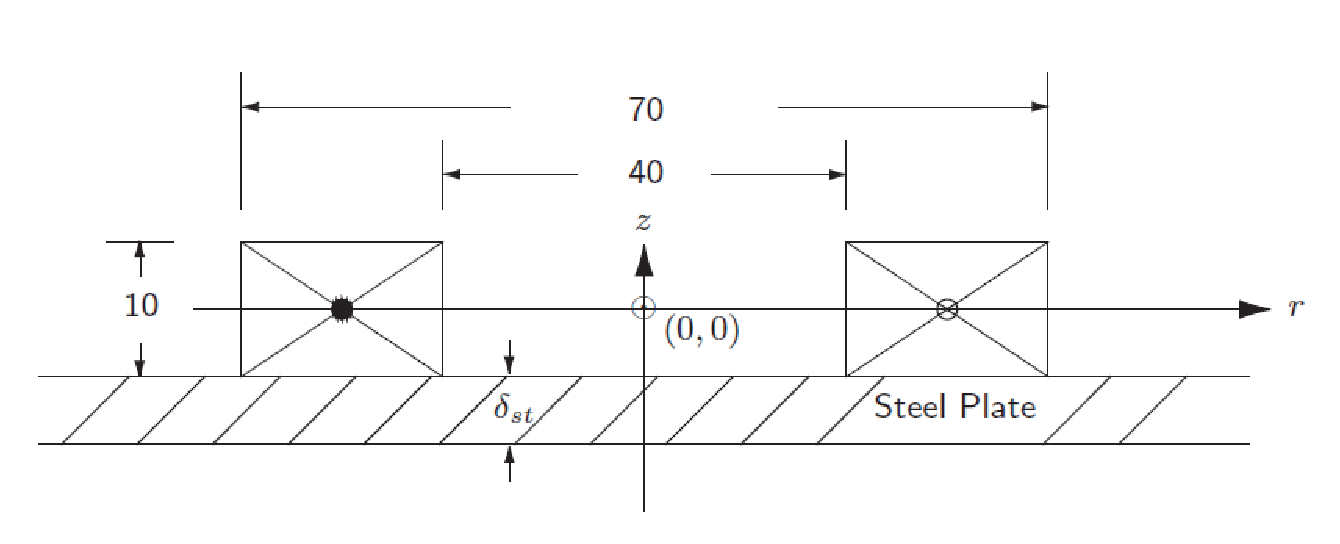
\includegraphics[scale=0.5]{chpt9/figs/fig9.6.eps}
	\caption{置于钢板上的超导线圈的截面图。尺寸单位为mm。}
\end{figure}


\begin{figure}
	\centering
	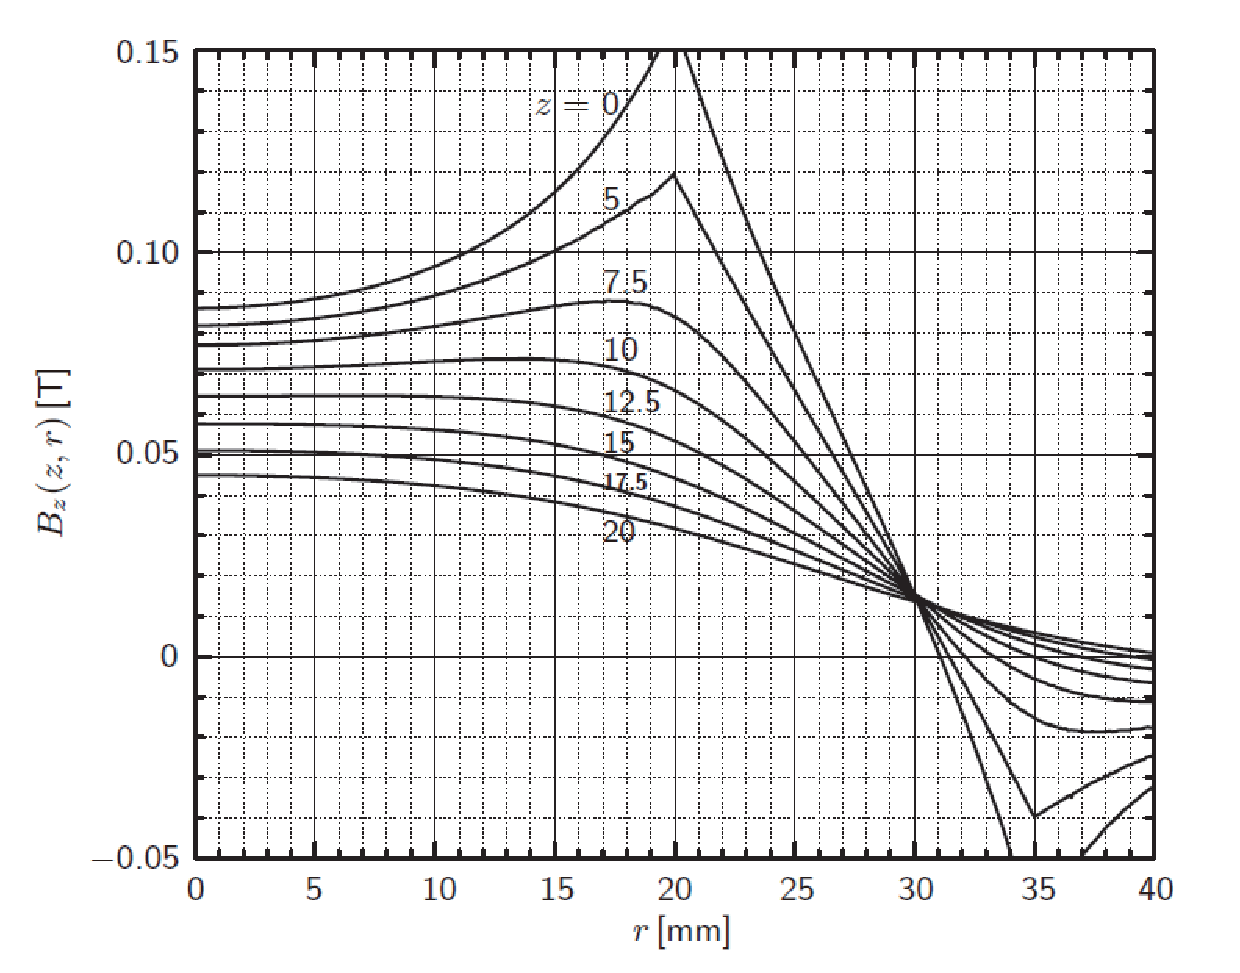
\includegraphics[scale=0.5]{chpt9/figs/fig9.7.eps}
	\caption{线圈通流25 A且无钢板时在$z$=0,5,7.5,10,12.5,15,17.5和20 mm时产生的磁场$B_z(z,r)$。
		$B_z(0,20)$=0.158 T,$B_z(0,35)$=-0.068 T。}
\end{figure}

\textbf{电感回顾}

如3.7节所讨论的,线圈的自感$L$可以由$\Phi$和$I$的关系给出:
\begin{align*}% page568 第1个
\Phi=LI \tag{3.78}
\end{align*}
其中$\Phi$是电流$I$时的总磁链:
\begin{align*}% page568 第2个
\Phi=2\pi\sum_{j=1}^{N}\int_{0}^{R_j}rB_z(z_i,r)dr \tag{9.1}
\end{align*}
式中,$R_j$是轴向距离$z=z_j$处的第$j$匝的半径。
明显这个积分手算起来很麻烦。但如今因为有了大量可以计算电感的程序,手算已不再必要。

这里我们针对图9.6所给的线圈,通过联立方程3.78和方程9.1的简化版本来计算电感的"说得过去精确"的值。
\begin{align*}% page568 第3个
L\simeq\frac{2N\pi}{I}\int_{0}^{a_2}B_z(z=0,r)dr \tag{9.2}
\end{align*}
方程9.2中,9.1的被积函数由一个仅涉及线圈中平面磁场的简单积积分项$B_z(0,r)$近似。
方程9.2给出了$L$的上限,因为并非所有$N$匝都在$r=a_2$交链;
实际上一些磁通仅交链于$a_1$内。
或许中间点$()a_1+a_2)/2$是径向积分限的一个很好的折中。


\subsubsection{Q/A B:钢板上的超导线圈}
\textbf{a) 线圈电感}\qquad 使用方程9.2和图9.7的$B_z(0,r)$图,计算线圈自感(无钢板)。
使用$B_z(0,r=20)$=0.158 T和$B_z(0,r=35)$=-0.068 T。

\textbf{解:}首先,$B_z(0,r)$和$B_z(0,r)r$的数据已列于表9.4。图9.8给出了$B_z(0,r)r$ vs. $r$曲线,
从中可知$\int B_z(0,r)rdr$和$\Phi$可以如下计算:
\begin{align*}% page569 第1个
\int_{0}^{a_2}B_z(0,r)dr&\simeq 38.0\ \mathrm{T mm^2}\mbox{图9.8中阴影部分}\\
&=3.80\times 10^{-5}\ \mathrm{Tm^2}\\
\Phi&=2\pi(3.80\times 10^{-5}\ \mathrm{Tm^2})\simeq 23.9\times 10^{-5}\ \mathrm{Tm^2}
\end{align*}
于是,
\begin{align*}% page569 第2个
L=\frac{N\Phi}{I}\simeq\frac{150(23.9\times 10^{-5}\ \mathrm{Tm^2})}{25\ \mathrm{A}}\simeq 1.43\ \mathrm{mH}
\end{align*}
该值比实际值1.33 mH大$\sim 10\%$。
由于在$-5\le z\le 5$ mm范围内,$B_z(0,r)$要比$B_z(z,r)$的平均值大,故方程9.2高估了$L$。
注意到,因为$B_z(0,r)r$在$r\simeq31$ mm和$a_2$之间积分为负,并且它与$(a_1+a_2)/2=27.5$ mm到
31 mm之间的积分制很接近,所以从0到$a_2$的积分最终与从0到$(a_1+a_2)/2$(上文提出的
更合适的积分限)之间的积分值近乎相等。

如3.7.2部分讨论的,对于一个参数为$a_1,\alpha,\beta,N$的螺管,其自感可由下式计算:
\begin{align*}% page569 第3个
L=\mu_oa_1N^2\mathcal{L}(\alpha,\beta) \tag{3.81}
\end{align*}
其中,$\mathcal{L}(\alpha,\beta)$如图3.14所示,仅依赖于$\alpha,\beta$。

由表9.3可知,$a_1$=0.02 m;$\alpha=70/40=1.75$;$\beta=10/40=0.25$;
$N=150$。
使用图3.14中的$\mathcal{L}(\alpha,\beta)$,当$\alpha=1.75$时,在$\beta=0.2$和$\beta=0.4$
之间做线性插值,我们有$\mathcal{L}(1.75,0.25)\simeq2.35$。于是:
\begin{align*}% page569 第4个
L\simeq(4\pi\times 10^{-7}\ \mathrm{H/m})(0.02\ \mathrm{m})(150)^2(2.35)=1.33\ \mathrm{mH}
\end{align*}
这与实际值完全相同。


表9.4.。。。。。。。。。。。。。。。。。


\begin{figure}
	\centering
	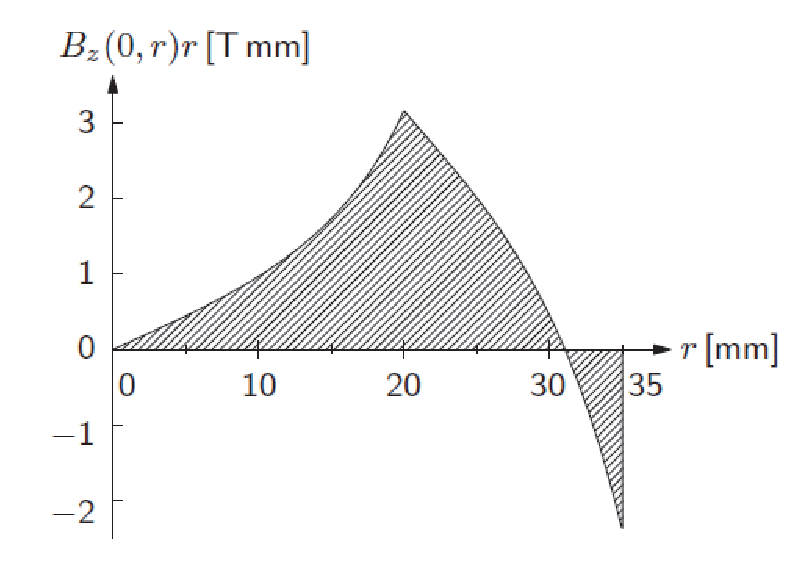
\includegraphics[scale=0.5]{chpt9/figs/fig9.8.eps}
	\caption{$B_z(0,r)r$ vs. $r$曲线。}
\end{figure}

\textbf{b) 钢板}\qquad 下面我们考虑钢板。
为了简化问题,我们首先假定钢板的磁导率无限大,即$\mu/\mu_o=\infty$。
接下来,为了模拟钢板对其上(即$z\ge -5$ mm)磁场的作用,
我们将钢板替换为一个和原线圈完全一样但至于板下的对称虚拟线圈,如图9.9所示。

通过证明虚拟线圈满足钢板在($r,z=-5\ \mathrm{mm}$)处的边界条件,
解释直接位于原线圈下的虚拟线圈能模拟理想钢板的效果。

\textbf{解:}$\mu/\mu_o=\infty$的理想钢板的边界条件是磁场切向分量(此处为轴向)在
板表面必须为零,即$B_z(z=-5\ \mathrm{mm})=0$。
也即,磁场必须以垂直钢板表面的形式穿入或传出。
与原线圈等同并且置于其下的线圈,根据对称性,可以满足上述边界条件。

\textbf{c) 钢板的场增强作用}\qquad 使用图9.9中的模型,计算线圈的中心场$B_z(0,0)$。
系统如图9.6,线圈载流为25 A。

\textbf{解:}由图9.7,没有钢板时,线圈通流25 A产生$[B_z(0,0)]_{w/o}\simeq 0.0863$ T。
有钢板时,我们必须加入中心点在$r=0$和$z=-10$ mm的虚拟线圈的贡献。
\begin{align*}%page570 第一个
[B_{z}(0,0)]_{with}&=[B_{z}(0,0)+B(z=10mm,0)]_{w/o}\\
&\simeq 0.0863+0.711\simeq 0.1574\ \mathrm{T}
\end{align*}
等式右侧的第二项即虚拟线圈的贡献。
可见,钢板不足以令上方区域磁场翻倍---仅在$z=-5$ mm处恰好翻倍。
钢板似乎令$z$=-5 mm下方区域的磁场翻折到了其上方区域。
理想钢板的下方,磁场为零。

\begin{figure}
	\centering
	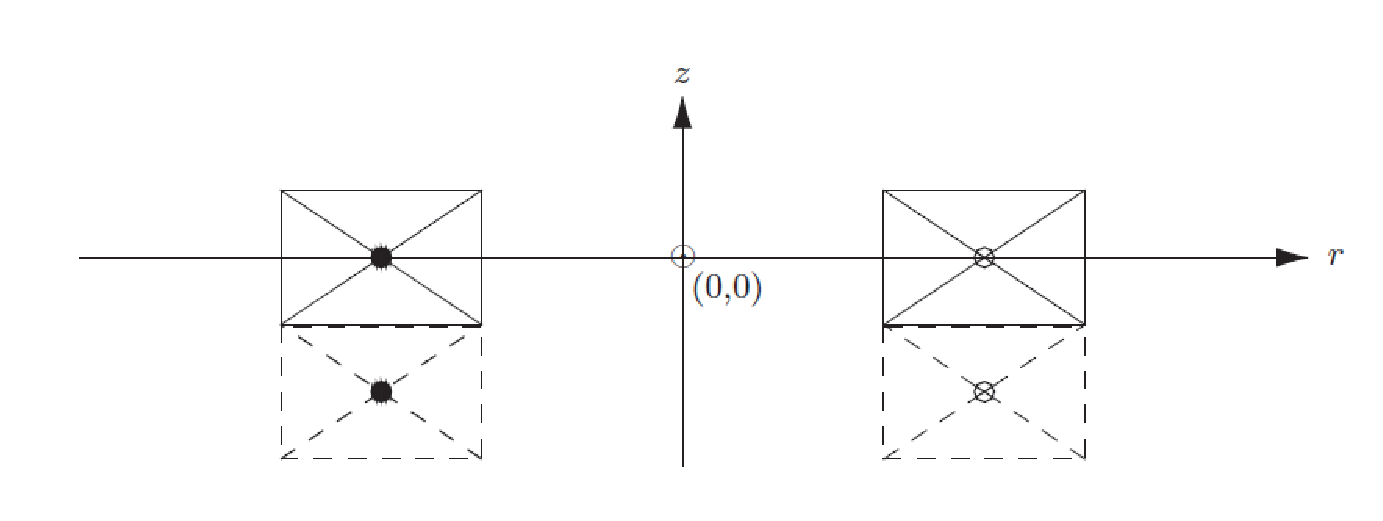
\includegraphics[scale=0.5]{chpt9/figs/fig9.9.eps}
	\caption{为建模钢板的效应而做的线圈安排。尺寸与图9.6相同。与原线圈等同的虚拟线圈置于
	原线圈下方,替代$\mu/\mu_o=\infty$的理想钢板。}
\end{figure}

\textbf{d) 钢板厚度}\qquad 为了确保我们对钢板的$\mu/mu_o\gg 1$假设有效,需保持钢板磁化强度$\mu_o M_{st}$小于1.25 T。计算所需钢板的最小厚度。

\textbf{解:}我们采用如下步骤:1) 假定钢板为



\begin{equation}%page571 第一个
\int_{0}^{r\pm}2B_{z}(z=5mm,r)r\quad dr\simeq7.22\times10^{-5}\ \mathrm{TM^{2}}(from\quad Fig.9.10)
\end{equation}
\begin{equation}%page571 第二个
\Phi_{r\pm}=2\pi(7.22\times10^{-5}\ \mathrm{Tm^{2}})\simeq45.4\times10^{-5}\ \mathrm{Tm^{2}}
\end{equation}
\begin{equation}%page571 第三个
\Phi_{st}=\pi r_{\pm}\delta_{st}(\mu_{o}M_{st})=\Phi_{r\pm}
\end{equation}
\begin{equation}%page571 第四个
\delta_{st}=\frac{\Phi_{r\pm}}{2r_{\pm}(\mu_{o}M_{st})}=\frac{45.4\times10^{-5}\ \mathrm{Tm^{2}}}{2\pi(0.03156m)(1.25T)}\simeq1.8mm
\end{equation}
\begin{equation}%page572 第一个
\int_{r\pm}^{r_{od}}B_{z}(r,z=5mm)d\quad dr>\sim(0.8)\int_{0}^{r\pm}B_{z}(r,z=5mm)r\quad dr
\end{equation}



\subsection{例C:平面HTS板的悬浮}

\subsubsection{Q/A C:平面HTS板的悬浮}
\begin{equation}%page574 第一个
F_{z}(z_{\ell})=2\pi R_{d}I_{s}B_{r}(z_{\ell},R_{d})\qquad(9.3a)
\end{equation}
\begin{equation}%page574 第二个
F_{z}(z_{\ell})=2\pi R_{d}I_{s}B_{r}(z_{\ell},R_{d})\qquad(9.3a)
\end{equation}
\begin{equation}%page574 第三个
\delta_{s}=\frac{H_{z}(z_{\ell},R_{d})}{J_{c}}=\frac{1}{J_{c}}[\frac{B_{z}(z_{\ell},R_{d})}{\mu_{o}}]\quad(a.1)
\end{equation}
\begin{equation}%page574 第四个
I_{s}=\delta_{d}\delta_{s}J_{c}=\delta_{d}[\frac{B_{z}(z_{\ell},R_{d})}{\mu_{o}}]\quad(a.2)
\end{equation}
\begin{equation}%page574 第五个
F_{z}(z_{\ell})=2\pi R_{d}\delta_{d}[\frac{B_{z}(z_{\ell},R_{d})B_{r}(z_{\ell},R_{d})}{\mu_{o}}]\quad(9.3b)
\end{equation}
\begin{equation}%page575 第一个
F_{z}(z_{\ell})=2\pi R_{d}\delta_{d}[\frac{B_{z}(z_{\ell},R_{d})B_{r}(z_{\ell},R_{d})}{\mu_{o}}]\qquad(9.36b)
\simeq\frac{2\pi(15\times10^{-3}\ \mathrm{m})(5\times10^{-3}\ \mathrm{m})(0.070\ \mathrm{T})(0.0181\ \mathrm{T})}{(4\pi\times10^{-7}\ \mathrm{H/m})}
\simeq0.475\ \mathrm{N}(\simeq48.5\ \mathrm{g})
\end{equation}
\begin{equation}%page575 第二个
m_{p}=\pi R^{2}_{d}\delta_{d\varrho}\\
=\pi(1.5\ \mathrm{cm})^{2}(0.5\ \mathrm{cm})(6.4\ \mathrm{g/cm^{3}})\simeq23g
\end{equation}
\begin{equation}%page575 第三个
\delta_{s}=\frac{H_{z}(z_{\ell},R_{d})}{J_{c}}=\frac{1}{J_{c}}[\frac{B_{z}(z_{\ell},R_{d})}{\mu_{o}}]\qquad(a.1)
\simeq\frac{(0.070\ \mathrm{T})}{(10^{8}\ \mathrm{A/m^{2}})(4\pi\times10^{-7}\ \mathrm{H/m})}\simeq0.56\ \mathrm{mm}
\end{equation}
\begin{equation}%page575 第四个
I_{s}=\delta_{d}\delta_{s}J_{c}\qquad(a.2)\\
\simeq(5\times10^{-3}\ \mathrm{m})(0.56\times10^{-3}\ \mathrm{m})(10^{8}\ \mathrm{A/m^{2}})\simeq280A
\end{equation}
\begin{equation}%page576 第一个
k_{z}=-frac{\partial F_{z}(z,R_{d})}{\partial_{z}}|_{z_{\ell}}\quad(d.q)
\end{equation}
\begin{equation}%page576 第二个
k_{z}=-2\pi R_{d}\delta_{d}\{[\frac{B_{r}(z_{\ell},R_{d})}{\mu_{o}}]\frac{\partial B_{z}(z,R_{d})}{\partial_{z}}|_{\ell}+[\frac{B_{z}(z_{\ell},R_{d})}{\mu_{o}}]\frac{\partial B_{r}(z,R_{d})}{\partial z}|_{\ell}\}(9.4)
\end{equation}
\begin{equation}%page576 第三个
k_{z}\simeq-2\pi(15\times10^{-3}\ \mathrm{m})(5\times10^{-3}\ \mathrm{m})\\
\times[(\frac{0.181\ \mathrm{T}}{4\pi\times10^{-7}\ \mathrm{H/m}})(-5.2\ \mathrm{T/m})+(\frac{0.070\ \mathrm{T}}{4\pi\times10^{-7}\ \mathrm{H/m}})(1.1\ \mathrm{T/m})]\\
=-2\pi(75\times10^{-6}\ \mathrm{m^{2}})(\frac{10^{7}}{4\pi}\ \mathrm{m/H})(-0.0943\ \mathrm{T^{2}/M}+0.758\ \mathrm{T^{2}/m})\\
\simeq6.9\ \mathrm{N/m}
\end{equation}
\begin{equation}%page576 第四个
\nu=\frac{1}{2\pi}\sqrt{\frac{k}{m}}
\end{equation}
\begin{equation}%page576 第五个
\nu_{z}\simeq\frac{1}{2\pi}\sqrt{\frac{(6.9\ \mathrm{N/m})}{(23\times10^{-3}\ \mathrm{kg})}}\\
\simeq3\ \mathrm{Hz}
\end{equation}
\begin{equation}%page577 第一个
F_{x}(z_{\ell},R_{d})+F_{x}(z_{\ell},-R_{d})\propto-I_{s}(z_{\ell},R_{d})+I_{s}(z_{\ell},R_{d})B_{z}(z_{\ell},-R_{d})\\
=0
\end{equation}
\begin{equation}%page577 第二个
F_{x}(z_{\ell},R_{d}+\Delta x)+F_{x}(z_{\ell},-R_{d}+\Delta x)\propto-I_{s}(R_{d}+\Delta x)B_{z}(z_{\ell},R_{d}+\Delta x)\\
+I_{s}(-R_{d}+\Delta x)B_{z}(z_{\ell},-R_{d}+\Delta x)(f1.1)
\end{equation}
\begin{equation}%page577 第三个
F_{x}(z_{\ell},R_{d}+\Delta x)+F_{x}(z_{\ell},-R_{d}+\Delta x)\propto-I_{s}(R_{d})[B_{z}(z_{\ell},R_{d}+\Delta x)\\
-B_{z}(z_{\ell},-R_{d}+\Delta x)](f1.2)
\end{equation}



\begin{equation}% page578 f2.2
\Delta f_x(z,R_d)=2I_s\Delta y\frac{\partial B_z(z,r)}{\partial r}\mid_{R_d}\Delta x
\end{equation}
\begin{equation}% page578 第二个f2.2
\Delta F_x(z,R_d)=\pi R_dI_s\frac{\partial B_z(z,r)}{\partial r}\mid_{R_d}\Delta x
\end{equation}
\begin{equation}% page578第三个
k_x(z,R_d)=\frac{\Delta F_x(z,R_d)}{\Delta x}=\pi R_dI_s\frac{\partial B_z(z,r)}{\partial r}\mid_{R_d}
\end{equation}
\begin{equation}% page578 第四个
k_x(z_\ell,R_d)=2(15\times 10^{-3}\ \mathrm{m})(280\ \mathrm{A})(1.08\ \mathrm{T/m})\simeq 14.2\ \mathrm{N/m}
\end{equation}
\begin{equation}% page578 f2.4
\upsilon_x=\frac{1}{2\pi}\sqrt{\frac{k_x}{m_p}} 
\simeq\frac{1}{2\pi}\sqrt{\frac{14.2\ \mathrm{N/m}}{(23\times 10^{-3}\ \mathrm{kg})}}\simeq 4\ \mathrm{Hz}
\end{equation}
\begin{equation}% page579 3.112
P=\rho_{cd}J^2\lambda a_{1}^{3}2\pi\beta(\alpha^2-1) 
=\rho_{cd}\frac{(\lambda J)^2}{\lambda}a_{1}^{3}2\pi\beta(\alpha^2-1)
\end{equation}
\begin{equation}% page579 g.1
P=\frac{\pi\rho_{cd}(NI)^2(\alpha+1)}{2\lambda a_1\beta(\alpha-1)}
\end{equation}
\begin{equation}% page579 第三个
P_1=\frac{\pi(2.5\times 10^{-9}\ \mathrm{\Omega m})(150\times 25\ \mathrm{A})^2(1.75+1)}{2(0.785)(20\times 10^{-3}\ \mathrm{m})(0.25)(1.75-1)}\simeq 52\ \mathrm{W}
\end{equation}
\begin{equation}% page579第四个
P_2=\frac{\pi(2.5\times 10^{-9}\ \mathrm{\Omega m})(50\times 15\ \mathrm{A})^2(1.5+1)}{2(0.785)(10\times 10^{-3}\ \mathrm{m})(0.5)(1.5-1)}\simeq 3\ \mathrm{W}
\end{equation}
\begin{equation}% page579 h.1
\dot{Q}_\ell=\frac{P}{h_L}
\end{equation}
\begin{equation}% page579 最后一个
\dot{Q}_\ell=\frac{(55\ \mathrm{W})}{(161\ \mathrm{J/cm^3})}=0.34\ \mathrm{cm^3/s}=1224\ \mathrm{cm^3/h} 
\sim 1\ \mathrm{liter/h}
\end{equation}
\begin{equation}% page580 第一个
[B_z(z_\ell,R_d)]_{\mathrm{with}}=[B_z(z_\ell,R_d)+B_z(z\ell+10.0\ \mathrm{mm},R_d)]_{\mathrm{w/o}} 
\simeq(0.070\ \mathrm{T})+(0.036\ \mathrm{T})=0.106\ \mathrm{T}
\end{equation}
\begin{equation}% page580 第二个
[B_r(z_\ell,R_d)]_{\mathrm{with}}=[B_r(z_\ell,R_d)+B_r(z\ell+10.0\ \mathrm{mm},R_d)]_{\mathrm{w/o}} 
\simeq(0.018\ \mathrm{T})+(0.015\ \mathrm{T})=0.033\ \mathrm{T}
\end{equation}
\begin{equation}% page580 9.3b
F_z(z_\ell,R_d)=2\pi R_d\delta_d\left[\frac{B_z(z_\ell,R_d)B_r(z_\ell,R_d)}{\mu_o}\right] 
\simeq\frac{2\pi(15\times 10^{-3}\ \mathrm{m})(5\times 10^{-3}\ \mathrm{m})(0.106\ \mathrm{T})(0.033\ \mathrm{T})}{(4\pi\times 10^{-7}\ \mathrm{H/m})} 
\simeq 1.31\ \mathrm{N}(\simeq 134\ \mathrm{g})
\end{equation}



\section{例D:HTS“环形”磁体}

\subsubsection{Q/A D:HTS“环形”磁体}


\begin{equation}% page582 3.111e
B_z(0,0)=\mu_o\lambda Ja_1(\alpha-1)
\end{equation}
\begin{equation}% page582 第二个
\lambda J=\frac{B_z(0,0)}{\mu_oa_1(\alpha-1)}=\frac{(11.74\ \mathrm{T})}{(4\pi\times 10^{-7}\ \mathrm{H/m})(0.025\ \mathrm{m})(1.5-1)}=7.5\times 10^8\ \mathrm{A/m^2}
\end{equation}
\begin{equation}% page584 d.1
\frac{\pi}{3}(a_{2}^{2}+a_2a_1+a_{1}^{2})B_o\simeq\frac{\pi}{4}(D_{so}^{2}-D_{si}^{2})\mu_oM_s
\end{equation}


\section{HTS磁体}
\subsection{主要应用领域---HTS(和LTS)}



\subsection{HTS磁体前景}



\section{结语}
